\part{Aritmética y Álgebra}


\null\vfill
\begin{Huge}\begin{center}
I. Aritmética y Álgebra
\end{center}\end{Huge}

\vspace{1.5cm}


\begin{figure}[H]
	\centering
	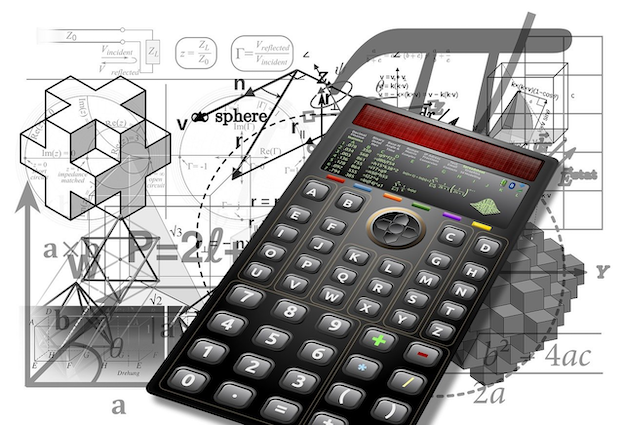
\includegraphics[width=.9\textwidth]{imagenes/part1.png}	
\end{figure}
\par
\vfill

\chapter{Números reales}
%\setlength{\parindent}{0cm}


\begin{tikzpicture}
	\fill [left color=red!50, right color=teal!50] (0,0) rectangle (6.5,.2);
	\fill [left color=teal!50, right color=blue!50] (6.5,0) rectangle (11.5,.2);
	\end{tikzpicture}

\vspace{15mm}


\begin{adjustwidth}{40pt}{40pt}
\begin{cuadro-gris}

	\begin{multicols}{2}
	$\triangleright \quad$  Intervalos, valor absoluto.
	
	$\triangleright \quad$  Radicales: racionalización.
	
	$\triangleright \quad$  Logaritmos.
	
	$\triangleright \quad$  Números combinatorios. Binomio de Newton.
	\end{multicols}
	
\end{cuadro-gris}
\end{adjustwidth}


\begin{figure}[H]
	\centering
	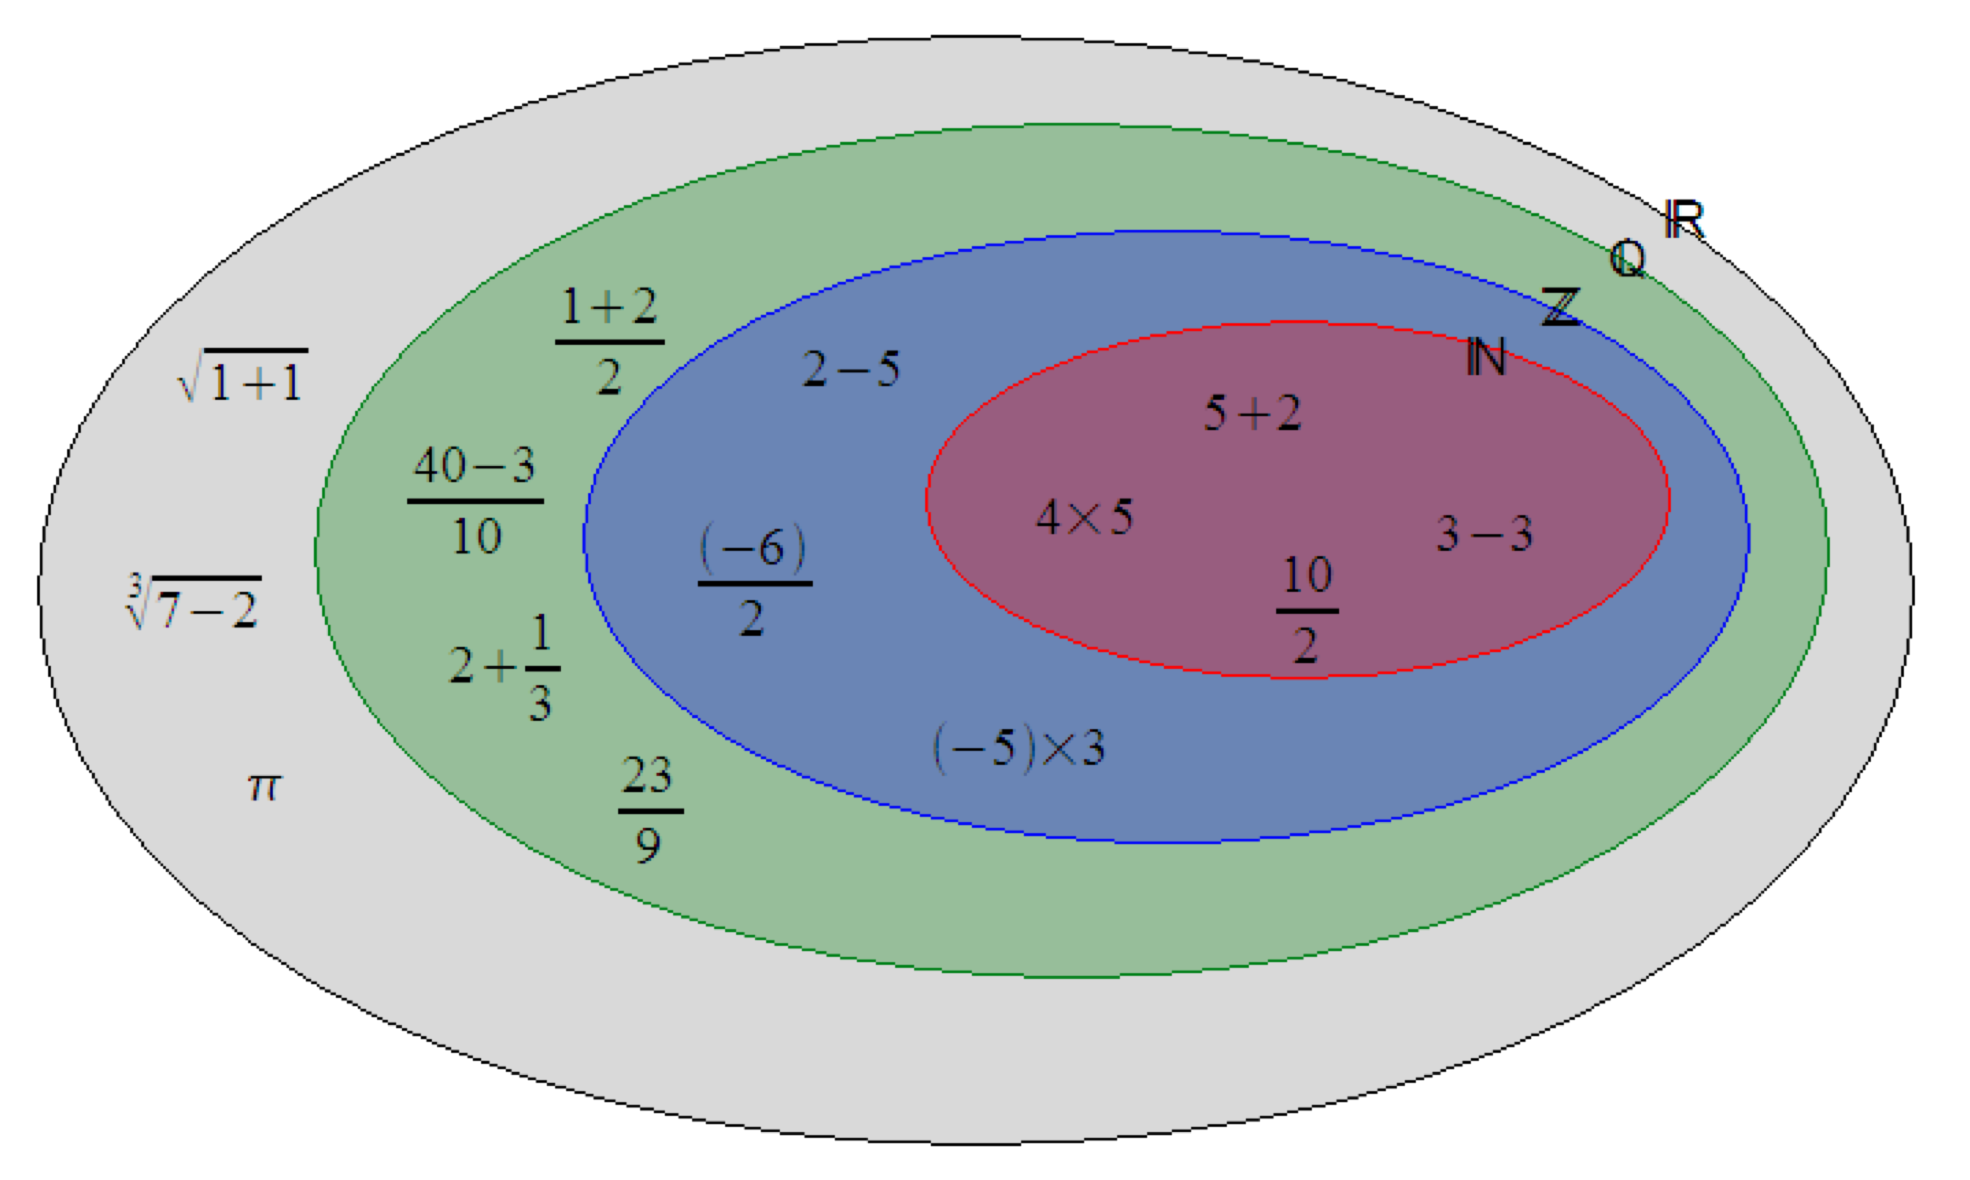
\includegraphics[width=.7\textwidth]{img-reales/reales00.png}	
\end{figure}


\section{Sucesivas ampliaciones de los conjuntos numéricos}

\begin{tikzpicture}
	\fill [left color=red!50, right color=teal!50] (0,0) rectangle (3.5,.1);
	\fill [left color=teal!50, right color=blue!50] (3.5,0) rectangle (7.5,.1);
	\end{tikzpicture}
\vspace{1cm}


Aunque la aparición de los distintos tipos de números no fue la que parecería lógica según sus relaciones de inclusión: primero los naturales, enteros, racionales hasta llegar a los reales;  permítaseme esta pequeña licencia narrativa a título meramente didáctico: \emph{``Y el hombre creó al número''}


\newpage %%%%%%%%%%%%%%%%%%%%%%%%%%%%%%%%%%

$\qquad$ %%%%%%%%%%%%%%%%%%%%%%%%%%%%%%%%%%

\begin{adjustwidth}{25pt}{25pt}

\begin{myexampleblock}{Y el hombre creó al número}
	
\vspace{3mm} 
\begin{multicols}{2}
Al principio, el ser humano sintió la necesidad de contar para, por ejemplo, saber la prole a la que tenía que alimentar (cuántas bocas tenía en la cueva). Estamos ante el nacimiento de los \emph{números naturales}, $\mathbb N$.
\begin{figure}[H]
	\centering
	
\includegraphics[width=.4\textwidth]{img-reales/reales01.png}	
\end{figure}
\end{multicols}

\vspace{3mm} 
\begin{multicols}{2}
\begin{figure}[H]
	\centering
	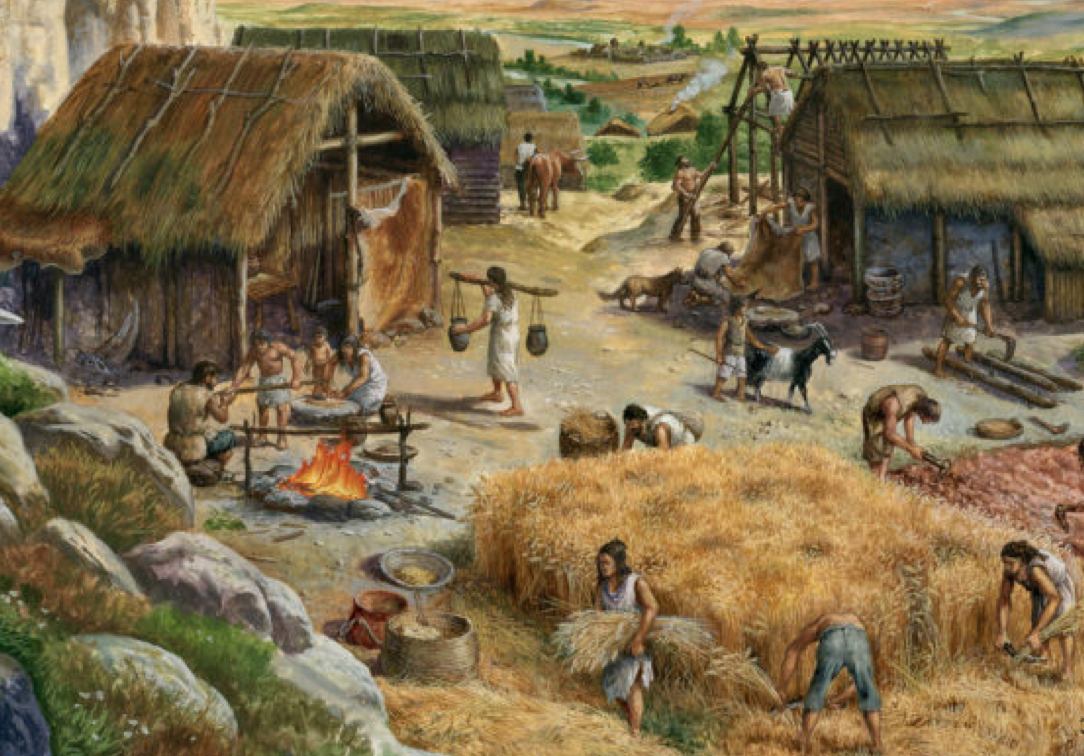
\includegraphics[width=.4\textwidth]{img-reales/reales02.png}	
\end{figure}
Pasó el tiempo y varios de ellos se juntaron en pequeñas tribus. Aparece el reparto del trabajo, lo que  conlleva la necesidad de restar: de la cantidad que te adeudo te pago esta cantidad, con lo que aún te debo esta otra. Surgen los \emph{números enteros}, $\mathbb Z$.
\end{multicols}	

\vspace{3mm} 
\begin{multicols}{2}
Las sociedades iban creciendo y aumentando sus temores a la oscuridad y a lo desconocido por lo que crean a sus primeras divinidades a las que adorar a cambio de protección y elevación de grandes templos. Tienen la necesidad de medir y ello lleva a dividir ampliando los números conocidos hasta entonces y aparecen los \emph{números racionales}, $\mathbb Q$.
\begin{figure}[H]
	\centering
	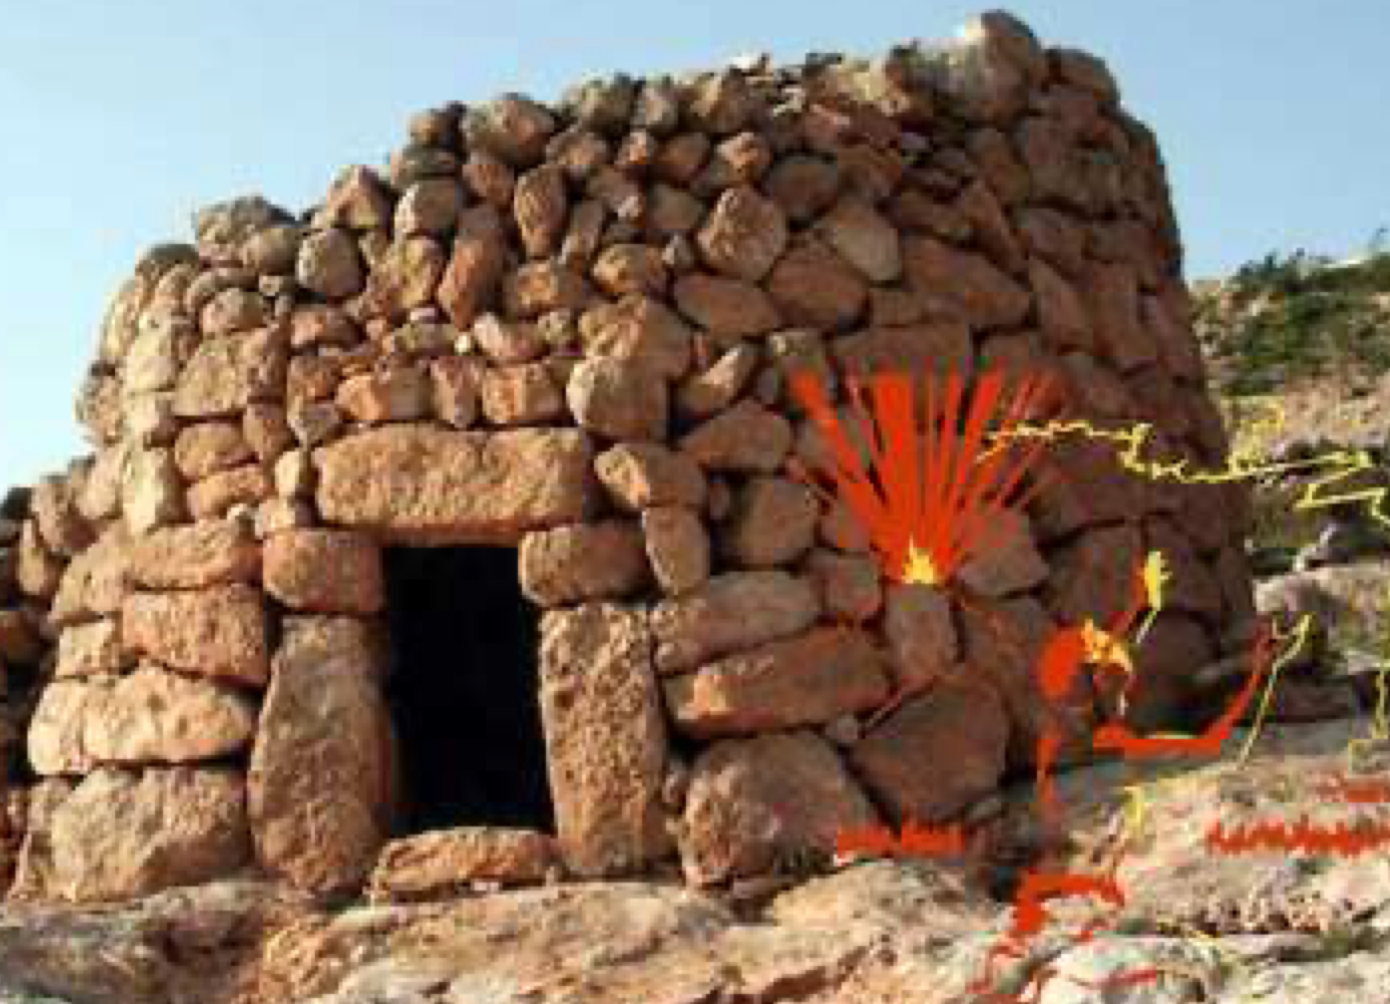
\includegraphics[width=.45\textwidth]{img-reales/reales03.png}	
\end{figure}
\end{multicols}

\vspace{3mm} 
\begin{multicols}{2}
\begin{figure}[H]
	\centering
	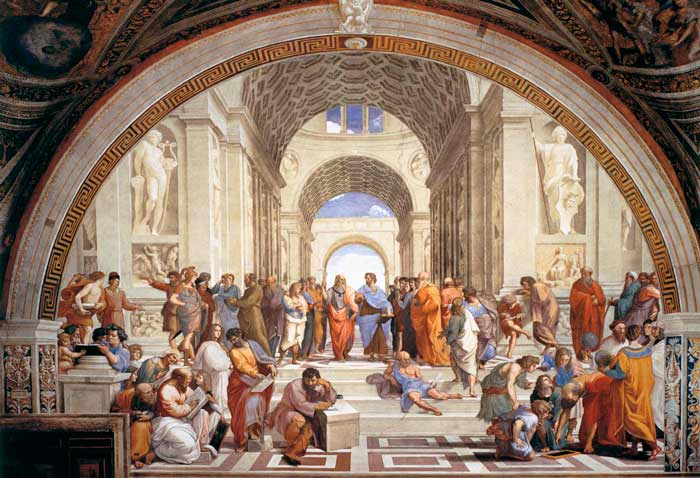
\includegraphics[width=.44\textwidth]{img-reales/reales04.png}	
\end{figure}
Profundizando en estos últimos números se dan cuenta de la existencia de otros verdaderamente extraños, no pueden tratarse como números racionales, son \emph{inconmensurables} (los llamados \emph{números irracionales}). La unión de ambos tipos de números dará lugar a los \textbf{\emph{números reales}}, $\boldsymbol{\mathbb R}$.
\end{multicols}

\end{myexampleblock}
\end{adjustwidth}

\newpage %%%%%%%%%%%%%%%%%%%%%%%%%%%%%%%%%%

\begin{multicols}{2}
En $\mathbb{N}$ podemos sumar y multiplicar, pero no restar ni dividir: $\ 2-5 \notin \mathbb{N}$ ($-3$ no es un número natural); $\ \frac 5 2 \notin \mathbb{N}$ ($\frac 5 2$ no es un número natural).

\begin{figure}[H]
	\centering
	
\includegraphics[width=.4\textwidth]{img-reales/reales05.png}	
\end{figure}

Este inconveniente se resuelve con los número enteros, $\mathbb{Z}$, ahora la resta no tiene ningún problema, $-3 \in \mathbb{Z}$ ($-3$ es un número entero). Continuamos, eso sí, sin poder dividir: $\frac 6 2 $ tiene sentido, da $3$, pero $\frac 2 6$ no lo tiene, no es un número entero.



Los números racionales, $\mathbb{Q}$, son la solución al problema, cualquier pareja de enteros que queramos dividir es posible, el resultado es siempre un número racional. Con números racionales ya podemos realizar las cuatro operaciones básicas: suma, resta, multiplicación y división (salvo, claro está, dividir por cero; esa operación no está definida).

Es sabido que la expresión decimal de cualquier número racional da como resultado un número periódico, pero no es difícil encontrar números decimales no periódicos: $0.101001000100001\cdots$ que no se pueden expresar como fracción (números racionales). Son los números irracionales los que, junto con los racionales, completan el conjunto de los números reales.
\end{multicols}

\begin{multicols}{2}
$$ \subrayado{ \mathbb N \subset \mathbb Z \subset \mathbb Q \subset \mathbb R }$$ 

$$\subrayado{ \mathbb R \supset \mathbb Q \supset \mathbb Z \supset \mathbb N }$$ 
\end{multicols}

$ \mathbb N=\{1,2,\cdots,817,\cdots \} \subset \mathbb Z \, ; \quad \mathbb Z=\{\cdots,-2,-1,\boldsymbol{0},1,2,3,\cdots \} \supset \mathbb N$

$ \mathbb Q=\left\{  \dfrac p q  \, / \,  p,q \in \mathbb Z \, , \ q>0  \ \wedge  \textcolor{gris}{(\text{y})} \ \   mcd ( |p|  ,q )=1  \right\}   \supset Z  \supset  N = \{\text{ fracciones  decimales periódicos } \}$
  
$\mathbb Q$ es \emph{denso}: entre dos racionales cualesquiera siempre se puede encontrar otro número racional (por ejemplo,  su media aritmética). No obstante, en la recta numérica (\emph{recta real}) hay infinitos puntos no ocupados por números racionales (decimales no periódicos, que no se pueden escribir como fracción).  A cada uno de estos puntos le corresponde un número irracional.  Ejemplos de número irracionales son  $\  0.1234\cdots \, ; \   1.010010001\cdots \, ; \ \sqrt{2}\, ; \ \pi \, ; \cdots$   

Los números irracionales se caracterizan porque: 
$\ a) \ $no pueden expresarse en forma de fracción, $\ b)\ $ su expresión decimal tiene infinitas cifras no periódicas. 

El conjunto de todos los números irracionales se designa por $\mathbb Q \smallsetminus \mathbb R$. 

\begin{adjustwidth}{25pt}{0pt}
$\triangleright\ \ $ Si $p$ no es cuadrado perfecto, $\sqrt{p}$ es irracional: $\sqrt{7}$ es irracional.

$\triangleright\ \ $ En general, cualquier raíz enésima no exacta es irracional: $\sqrt[5]{31}$ es irracional.

$\triangleright\ \ $ La operación de un número racional con uno irracional da un resultado irracional (excepto la multiplicación por cero): $3\cdot \sqrt{2}-4$ es irracional.

$\triangleright\ \ $ Irracionales famosos:  $\pi,\, \phi, \, e,\, \cdots$
\end{adjustwidth}

La unión de los números racionales y los irracionales forman los números reales. El conjunto de los números reales se designa por $\mathbb R$. \emph{Los números reales llenan la recta numérica por eso se la llama recta real}.  $\ \mathbb R$ es completo: a cada punto de la recta le corresponde un  único número real y cada número real se representa por un único punto en la recta (correspondencia biunívoca).

$$\boxed{ \ \boldsymbol{ \subrayado{\mathbb N \subset \mathbb Z \subset \mathbb Q \subset \mathbb R} } \ }$$

$$\text{Números Reales }
\begin{cases}
\ \text{ Racionales } 
	\begin{cases}
	\text{ Enteros } 
		\begin{cases}
		\text{ Naturales } \, : 1,\, 2,\, 	\cdots ,\, 139,\ \cdots \\
		\text{ No positivos }\, : \ -17,\,  0,\, \cdots
		\end{cases}
	\\
	\text{ Fraciones } \, : \ \dfrac 2 3,\, 7.0\widehat{34},\, \cdots
	\end{cases}	
\\
\ \text{ Irracionales }\, : \ \sqrt{2},\ \sqrt[3]{5},\ \pi,\ \cdots 
\end{cases}$$


\vspace{5mm}

\begin{myexampleblock}{ $\sqrt{2}$ es irracional.\hspace{5mm} \emph{Demostración por reducción al absurdo}}


\color{teal}\rule{250pt}{0.1pt}

\begin{footnotesize}{\textcolor{teal}{La `demostración por reducción al absurdo' es uno de los métodos de demostración más usados en matemáticas. Se parte por suponer como hipótesis la falsedad de lo que se quiere demostrar y, mediante una concatenación de inferencias lógicas, se pretende llegar a una contradicción, un absurdo. Al llegar a una contradicción, se concluye que la hipótesis de partida (que se había supuesto falsa al principio) ha de ser verdadera.}}\end{footnotesize}
\vspace{-5mm}
\begin{flushright}
\color{teal}\rule{250pt}{0.1pt}	
\end{flushright}
 
\color{black}

\normalsize{Supongamos} que $\sqrt{2}$ no fuese un número irracional, que fuese racional. Acabaremos llegando a una contradicción por lo que podremos concluir que, necesariamente, $\sqrt{2}$ es irracional.

\vspace{2mm} Si $\sqrt{2}$ es racional, deberán existir dos enteros $p,\, q \in \mathbb Z$, de modo que podamos escribirlo como una fracción:
$\ \sqrt 2=\dfrac p q\, , \ $ siendo $p \text{ y } q$ primos entre sí (co-primos) para que la fracción sea irreducible.

\vspace{2mm} Elevando al cuadrado, $\ 2=\dfrac {p^2}{q^2} \ \Rightarrow \ 2q^2=p^2\, \ $ de lo que deducimos que $p^2$ ha de ser par, múltiplo de $2$ y, necesariamente, también lo será $p$. Podremos escribir $p=2k$, para algún $k\in \mathbb Z$

\vspace{2mm} Sustituyendo en la expresión anterior, $ 2=\dfrac{(2k)^2}{q^2}=\dfrac{4k^2}{q^2} \ \Rightarrow \  q^2=2k^2\ $ y obtenemos que $q^2$ también es par, así como también lo será $q=2l$, para algún $l \in \mathbb Z$.

\vspace{2mm} Podremos escribir $\ \sqrt{2}=\dfrac p q = \dfrac{\cancel{2} k}{\cancel{2} l}=\dfrac k l \ $ lo que entra en contradicción con la hipótesis de partida, que $\dfrac p q$ era fracción irreducible.

\vspace{2mm} Conclusión: $º \sqrt{2}$ es \emph{irracional} \footnote{ $\ \ $ El símbolo $\blacksquare$  es típico al final de las demostraciones en matemáticas y significa \emph{``quod erat demostrandum'', `como queríamos demostrar'}, indica que la demostración ha acabado} \QED
 
\vspace{5mm}
	
\end{myexampleblock}

\vspace{5mm}
\color{teal}
\rule{250pt}{0.1pt}	

?`Cuántos números hay?. En realidad la cantidad de números naturales es infinita, pero hay infinitos más grandes que otros. Al infinito de los números naturales se le llama \emph{infinito numerable} y se puede demostrar que en los números enteros y los racionales hay también un infinito numerable de ellos. Pero números irracionales (y por lo tanto reales) hay más, ya no forman un infinito numerable y se le llama \emph{potencia del continuo}.
\vspace{-5mm}
\begin{flushright}
\rule{250pt}{0.1pt}	
\end{flushright}
\color{black}
\vspace{5mm}

\begin{miejercicio}

Clasifica los siguientes números según el menor conjunto numérico al que pertenezcan:

\begin{table}[H]
\centering
\begin{tabular}{|c|c|c|c|c|c|c|c|}
\hline
$\quad \sqrt{3} \quad$ & $\quad 5 \quad$  & $\quad -2 \quad$ & $\quad 4.5 \quad$ & $\quad 7.\widehat 3 \quad$ & $\quad -\sqrt[3]{6} \quad$ & $\quad \sqrt{64} \quad$ & $\quad \sqrt[3]{-27} \quad$  \\ \hline \hline
$\mathbb{R}$ & $\mathbb{N}$ & $\mathbb{Z}$ & $\mathbb{Q}$ & $\mathbb{Q}$ & $\mathbb{R}$ & $\mathbb{N}$ & $\mathbb{Z}$     \\ \hline
\end{tabular}
\end{table}
\end{miejercicio}

\begin{miejercicio}

Da tres números racionales y tres irracionales comprendidos entre $5.1112\cdots$ y $5.1222....$

\rule{250pt}{0.1pt}

\vspace{3mm}
$\mqty{
\ \bold{5.11}12\cdots \\
\ \bold{5.12}22\cdots 
} \ \to \ 5.11X \ (X>1)\ \to \ $ Problema abierto, por ejemplo,

$\to \ 
\begin{cases}
\text{ racionales: }	\ & 5.115; \ 5.1155;\, 5.115\widehat 3 
\\
\text{ irracionales: } \ & 5.1151234\cdots;\ 5.115101001000\cdots;\ 5.115101101110\cdots
\end{cases}
$
 	
\end{miejercicio}


%%%%%%%%%%%%%%%%%%%%%%%%%%%%%%%%%%%%%%%%%%%%%%%%%%%%%%%%%%%%%%%%%%%%%%%%%%%%%%%%%%%%%%%%%%%%%%%%%%%%%%%%%%%%%%%%%%%%%%%%%%%%%%%%%%%%%%%%%%
\vspace{10mm}
\subsection{Valor absoluto}

\begin{tikzpicture}
	\fill [left color=red!50, right color=teal!50] (0,0) rectangle (3.5,.01);
	\fill [left color=teal!50, right color=blue!50] (3.5,0) rectangle (7.5,.01);
	\end{tikzpicture}
\vspace{0.5cm}
	
	\begin{definition}[ Valor Absoluto] 
	
	El valor absoluto de un número real $\, x\in \mathbb R\, $ se define como el número:
	\begin{multicols}{2}
	$\quad$
	
	\begin{equation*}
		|x|=
		\begin{cases} 
		\;\;  x &\mbox{ si } x\ge 0 \\ 
		\; -x & \mbox{ si } x<0 
		\end{cases}
	\end{equation*}	
	
	$\quad$
	\begin{figure}[H]
	\centering
	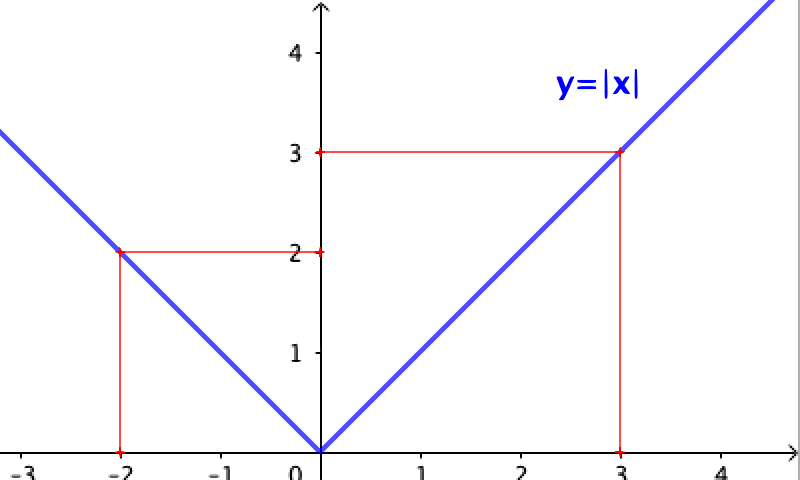
\includegraphics[width=.3\textwidth]{img-reales/reales06.png}	
\end{figure}
	\end{multicols}
	\end{definition}

El valor absoluto es, en matemáticas el \textit{gran positivizador}: $\ |3|=3;\ \ |-2|=-(-2)=2; \ \ |0|=0$.
	
%%%%%%%%%%%%%%%%%%%%%%%%%%%%%%%%%%%%%%%%%%%%%%
 
 Obsérvese que para eliminar las barras del valor absoluto nos tenemos que fijar en el signo de lo que vaya dentro de las barras del valor absoluto. Si es positivo queda igual y si es negativo, cambiamos el signo de lo que vaya dentro.

 El problema se nos presenta cuando no conozcamos el signo. Por ejemplo, resolver la siguiente ecuación con valor absoluto $|x|=3$.
 
Para resolverla, lo primero es quitar el valor absoluto. Debemos conocer el signo de lo de dentro, de $x$. Como no lo sabemos, no podemos quitar el valor absoluto. En estos casos se supone que lo de dentro del valor absoluto puede presentar los dos signos, luego el problema tiene doble solución:

$\begin{cases}
\text{ si } x>0 \ (\text{positivo})\ \to |x|=x=3  & \Rightarrow \boldsymbol{x=3}
\\ 
\text{ si } x<0 \, (\text{negativo})\, \to |x|=-x=3  & \Rightarrow \boldsymbol{x=-3}
\end{cases} \qquad  \boldsymbol{ |x|= 3 \ \Leftrightarrow \ x=3 \, \vee \textcolor{gris}{(\text{o})} \ x=-3 }$

\vspace{5mm}
\begin{miejercicio}

Resuelve la ecuación: $\qquad \left| \dfrac{2x-3}{4} \right| = 5$	

\vspace{2mm}
\rule{250pt}{0.1pt}
\vspace{2mm}

$\left| \dfrac{2x-3}{4} \right| = 5 \Leftrightarrow \begin{cases}
\ \dfrac{2x-3}{4} = 5 \to \ \ 2x-3=\ 5\cdot 4\ \to 2x=\ 23 & \Rightarrow \boldsymbol{x=23/2}
\\
\ \dfrac{2x-3}{4} = -5 \to  2x-3=-5\cdot 4\to 2x=-17 & \Rightarrow \boldsymbol{x=-17/2}
 \end{cases}$


\end{miejercicio}


\vspace{5mm}
\begin{theorem}[ Propiedades del valor absoluto] 	
	
	\begin{enumerate}
		\item $\quad  |-x|=|x|$
		\item $\quad |xy|=|x|\cdot|y|$
		\item $\quad \left| \dfrac x y \right| = \dfrac {|x|}{|y|}$
		\item $\quad |x|\le y\;  \mbox{ es equivalente a } -y\le x \le y $
		\item $\quad |x+y|\le|x|+|y|\qquad$ \emph{Desigualdad Triangular}
	\end{enumerate}
\end{theorem}	

\begin{multicols}{2}
Es sencillo comprobar con ejemplos que las afirmaciones anteriores son ciertas, las demostraciones rigurosas se dejan para cursos superiores. 

Una figura como demostración sin palabras de la desigualdad triangular. Se entiende por $|\vec a|$ al módulo (tamaño) del vector (segmento orientado) $\vec a$.
	
\begin{figure}[H]
	\centering
	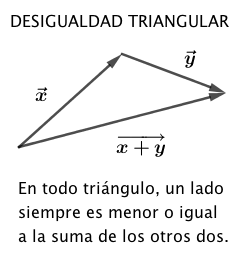
\includegraphics[width=0.3\textwidth]{img-reales/reales07.png}
\end{figure}
\end{multicols}

		
\begin{definition} [ Distancia entre números reales]

Llamamos \emph{distancia} $d$ entre dos números $x,y:\quad$ $ d(x,y)=|y-x|\, , \quad \forall x,y \in \mathbb R \ $ \footnote{ El símbolo $\ \forall \ $  se lee \emph{`para todo'}: $\ \forall x,y\in \mathbb R$ significa `para todo $x$ e $y$ números reales', es decir, para $x$ e $y$ dos números reales cualesquiera.}
\end{definition}
		


\begin{theorem}[ Propiedades de la distancia]

Se cumplen las siguientes propiedades para las distancias ($\forall$ se lee `para todo'). 
		
\begin{enumerate}[D1]
	\item  $\qquad \forall x \in \mathbb R:\; \ \ d(x,x)=0 $
	\item  $\qquad \forall x, y \in \mathbb R:\; \ \ d(x,y)=d(y,x)$
	\item  $\qquad \forall x, y, z \in \mathbb R:\; \ \ d(x,z) \le d(x,y)+d(y,z)$
\end{enumerate}
\end{theorem}		
		
\underline{Demostración}: En este caso, por su sencillez, demostramos el teorema para que el lector/a vaya acostumbrándose a ellas.

$\triangleright \ D1:\quad d(x,x)=|x-x|=|0|=0$ \QED

$\triangleright \ D2:\quad d(x,y)=|y-x| \mqty{ * \\ \leq \\ \ } |-(y-x)|=|x-y|=d(y,x)$ \QED

$*\ $ Hemos usado la propiedad $1.\, $ del valor absoluto, $|z|=|-z|$. 

$\triangleright \ D2:\quad d(x,z)=|z-x|=|z-y+y-x|\mqty{ ** \\ \leq \\ \ }|z-y|+|y-x|=d(y,z)+d(x,y)$ \QED

$**\ $ En la última demostración hemos usado la `desigualdad triangular'. 

Los símbolos $\blacksquare$ significan que la demostración ha acabado y se leen \emph{`como queríamos demostrar'} (quod erat demonstrandum, en latín). En textos antiguos aparece como siglas, \emph{q.e.d.}

\vspace{5mm}
\subsection{Intervalos}

\begin{tikzpicture}
	\fill [left color=red!50, right color=teal!50] (0,0) rectangle (3.5,.01);
	\fill [left color=teal!50, right color=blue!50] (3.5,0) rectangle (7.5,.01);
	\end{tikzpicture}
\vspace{.5cm} %%%%%%%%%%%%%%%%%%%%%%%
		
	
\begin{definition}[ Intervalos] 
	
Un intervalo es un subconjunto $I \subset \mathbb R$ tal que $\forall u,w \in I\; $, con $u\neq w\; $, y $\forall v \in \mathbb R\; $ con $u<v<w\; $ se cumpla que $v\in I$. Los intervalos pueden ser abiertos, cerrados y semiabiertos.\end{definition}

Esta es la definición rigurosa, necesaria en matemáticas, pero lo podemos entender como un subconjunto de números reales que se encuentran entre dos valores que delimitan un extremo inferior y otro superior. Los intervalos pueden ser abiertos o cerrados en cada uno de sus extremos, incluso pueden ser no acotados.

$\forall a,b \in \mathbb R\, ,\ $ se definen:
	
		\begin{figure}[H]
			\centering
			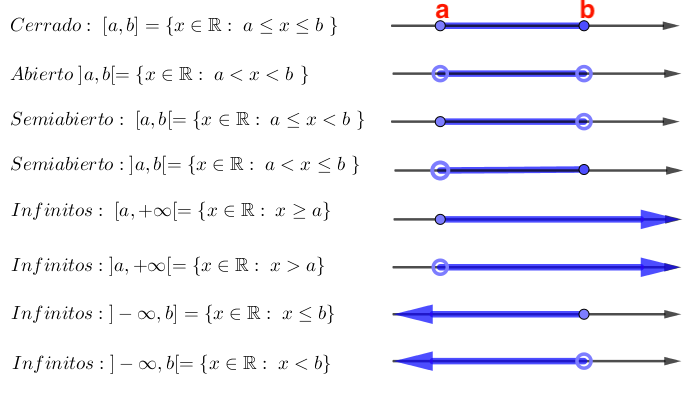
\includegraphics[width=0.8\textwidth]{img-reales/reales08.png}
		\end{figure}

\begin{miejercicio}

Da como notación de intervalos los siguientes subconjuntos de $\mathbb R$:

$a)\ \{ x\in \mathbb R \, / \, -2\leq x < 3 \} $ \footnotesize{(número reales tales que estén comprendidos entre -2 -inclusive- y 3 -exclusive-)} \normalsize{;} $\ \ b)\ \ $ número mayores que $-1$.

\vspace{3mm} \rule{250pt}{0.1pt}
\vspace{3mm}

Basta con representar los conjuntos en la recta real para determinar los intervalos buscados. Hemos tomado por convenio el dibujar un punto relleno para representar las igualdades ($\leq,\ \geq$) y un punto vacío para las desigualdades estrictas ($<,\ >$).

\begin{figure}[H]
			\centering
			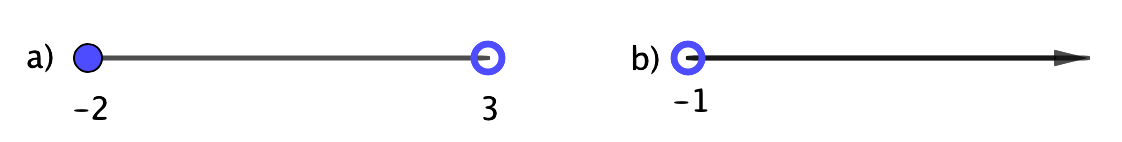
\includegraphics[width=0.7\textwidth]{img-reales/reales10.png}
		\end{figure}
		
Solución: $\quad a)\ \ [-2,3[\, ; \qquad b)\ \ ]-1,\infty]$
\end{miejercicio}

\vspace{5mm}


\begin{miejercicio}

Calcula :  $\qquad a) \ \ [1,4] \, \cup \, ]2,5[\, ; \qquad \qquad b)\ \ [1,4] \, \cap \, ]2,5[	$

\vspace{3mm}
\rule{250pt}{0.1pt}
\vspace{3mm}

Basta con representar los intervalos en la recta real, uno de ellos lo rayamos en vertical y el otro en horizontal. La unión $(\cup)$ será toda la zona rayada y la intersección $(\cap)$
 la zona con ambas rayas (zona cruzada).
 
 \begin{multicols}{2}
\begin{figure}[H]
			\centering
			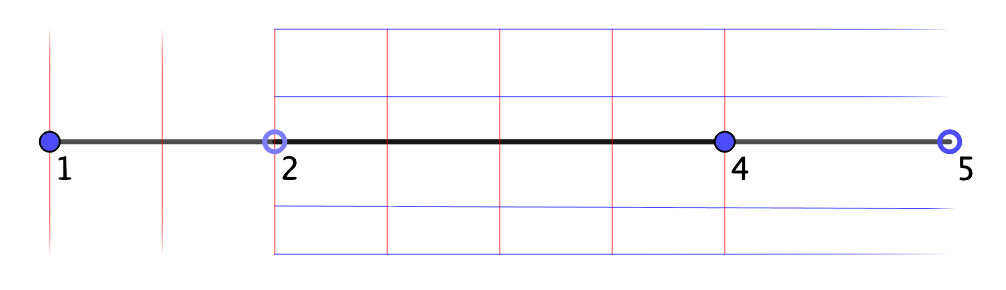
\includegraphics[width=0.45\textwidth]{img-reales/reales11.png}
		\end{figure} 	
		$\qquad \qquad a) \quad [1,5[$
		
		$\quad$
		
		$\qquad \qquad b) \quad ]2,4]$
 \end{multicols}

 
 \end{miejercicio}
	
\vspace{1cm}		
\begin{definition}[ Entorno]: 
	
$\forall a \in \mathbb R, \; \forall r \in \mathbb R^{+} \ $\footnote{ $\ \mathbb R^+\, \equiv ]0,+\infty[\, , $ son los números positivos. }
se define el \emph{entorno} de centro $a$ y radio $r$ como todos los números reales cuya distancia a $a$ sea menor que $r$:

$$\quad E_r(a)=\{ \forall x \in \mathbb R \;  / \; d(x,a)<r \}=]a-r,a+r[$$
		
\vspace{3mm} Se define el \emph{entorno reducido} de centro $a$ y radio $r$ como todos los números reales cuya distancia a $a$ sea menor que $r$, excluyendo al número $a$:
		
$$\quad E^*_r(a)=\{ \forall x \in \mathbb R \;  / \; 0<d(x,a)<r \}=]a-r,a+r[\smallsetminus \{a\} \small{\textcolor{gris}{\ = ]a-r,a[\cup ]a,a+r[}}$$
			
\end{definition}

\vspace{4mm} 

	
	\begin{myalertblock} {Valores Absolutos e Intervalos.}
		\begin{multicols}{2}
		\begin{itemize}
			\item $|x|=k \longleftrightarrow x=\pm k$
			\item $|x|<k \longleftrightarrow -k<x<k \longleftrightarrow ]-k,k[$
			\item $|x|\le k \longleftrightarrow -k\le x\le k \longleftrightarrow [-k,k]$
			\item $|x|> k \longleftrightarrow x>k\quad o \quad x<-k$
			\item $|x|\ge  k \longleftrightarrow x\ge k\quad o \quad x\le -k$
		\end{itemize}
		\begin{figure}[H]
			\centering
			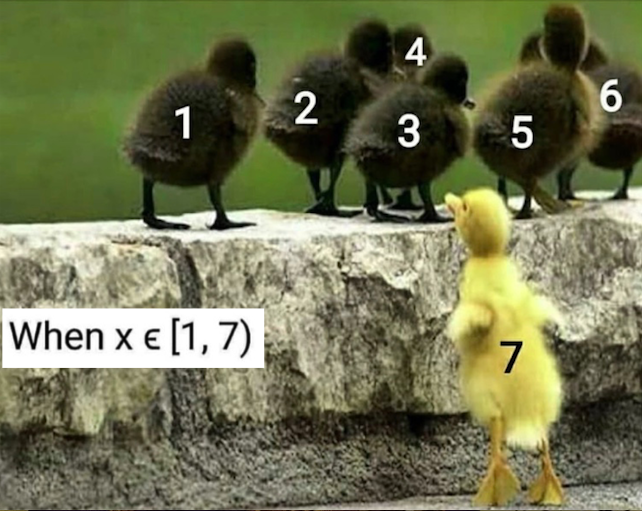
\includegraphics[width=0.4\textwidth]{img-reales/reales09.png}
		\end{figure}
		\end{multicols}
	\end{myalertblock}
		
\vspace{4mm} \underline{Nótese que}:  \hspace{.5cm} en el intervalo $[2,5[$, $2 \in [2,5[$, sin embargo, $5 \notin [2,5[$.

\vspace{4mm}\underline{Nota}: \hspace{.5cm} En muchos textos, los intervalos abiertos aparecen con paréntesis en lugar de corchetes, $]a,b[\equiv (a,b);\ [c,d[\equiv [c,d)\, . $ Nosotros continuaremos utilizando los corchetes para evitar la posible confusión con la notación para las coordenadas cartesianas de puntos en el plano.

\vspace{1cm}
\section{Radicales}

\begin{tikzpicture}
	\fill [left color=red!50, right color=teal!50] (0,0) rectangle (3.5,.1);
	\fill [left color=teal!50, right color=blue!50] (3.5,0) rectangle (7.5,.1);
	\end{tikzpicture}
\vspace{0.5cm}

\begin{definition}[ Radical ]

Se llama \emph{raíz $n$-sima} de un número real $a$, que representamos por $\sqrt[n]{a}$, al número real $b$ tal que $b$ sea la potencia $n$-sima de $a$:

$$ \boxed{ \ \boldsymbol{\sqrt[n]{a}\ = \ b \ \leftrightarrow \ b^n\ = \ a } \ }\qquad a,b\in \mathbb R,\quad n\in \mathbb N,\ n>1 $$

$\sqrt[n]{a}\,:\ $ radical; $\qquad a \, : \ $ radicando; $\qquad n\,: \ $ índice de la raíz	
\end{definition}

Si no aparece $n$ explícitamente se supondrá que es un $2$: raíces cuadradas.

\vspace{5mm} Dado un número real $a$ cualquiera y un natural mayor que uno, $n$, cualquiera, la ecuación $\ x^n=a\, $ tiene:

\vspace{-2mm}  \begin{itemize}
\vspace{-2mm} \item Dos soluciones, $+\sqrt[n]{a}$	 y $-\sqrt[n]{a}$ si $n$ es par y $a$ positivo.  
\vspace{-2mm} \item Las raíces pares de números negativos no existen.
\vspace{-2mm} \item Una solución única si $n$ es impar, siendo ésta positiva si lo es $a$ y negativa en caso contrario. 
\end{itemize}

$\sqrt[4]{16}=2;\ \ -\sqrt{25}=-5 ; \ \ \nexists \sqrt[4]{-1}; \ \ \sqrt[3]{-8}=-2; \ \ \sqrt[5]{1}=1 \qquad $ \textcolor{gris}{$\nexists$ se lee  \emph{`no existe'}}.

\vspace{5mm}
\begin{myalertblock}{Ambigüedad en el signo de la raíz cuadrada.}

Se considera que $\sqrt{x},\ x>0$ tiene solo un signo válido, el positivo. Así, escribiremos $\sqrt{4}=2;\ -\sqrt{4}=-2$

\vspace{2mm} Al resolver ecuaciones del tipo $(x+3)^2=16$,

\vspace{2mm} 
\begin{small}
$\begin{cases}
\text{ mal procedimiento: } \ & \\
\ (x+3)^2=169 \ \to \ \sqrt{(x+3)^2}=\sqrt{169} \ \to \ x+3=\pm 13 \ \to \ \begin{cases} \ x=10 \\ \ x=-16 \end{cases}
\\
\text{ procedimiento correcto: } \ & \\
\ (x+3)^2=169 \ \to \ \sqrt{(x+3)^2}=\sqrt{169} \ \to \ |x+3|=13 \ \to \ x+3=\pm 13  \ \to \ \begin{cases} \ x=10 \\ \ x=-16 \end{cases}
\end{cases}$
\end{small}
	
\end{myalertblock}



\vspace{5mm}\begin{definition}[ Potencias de exponente racional]

\begin{large}
$$\boldsymbol{ \sqrt[n]{a} \ = \ a^{\frac 1 n} \quad \longrightarrow \quad \sqrt[n]{a^m}\ = \ a^{\frac m n} } \qquad \qquad (\sqrt[n]{a})^m=\sqrt[n]{a^m} \ \ ( \circledast )$$	\end{large} 

\normalsize{Las} potencias de exponentes racionales son radicales siendo la base el radicando, el denominador del exponente de la potencia el índice de la raíz, el numerador el exponente del radicando.
\end{definition}

\textcolor{gris}{Justificación: $\qquad a^{1/n}=b \ \to \ (a^{1/n})^n=a=b^n \ \to \ b=\sqrt[n]{a}=a^{1/n}$}

$ \circledast \ $ En realidad, esta propiedad solo es cierta si existe $\sqrt[n]{a}$ y también $\sqrt[n]{a^m}$. Por ejemplo, $\ (\sqrt{-1})^2 \neq \sqrt{(-1)^2}$, la primera expresión no existe.

\vspace{5mm}\begin{miejemplo}

$\qquad 125^{\frac 1 3 }= \sqrt[3]{125}=5; \qquad \qquad 16^{\frac 3 4}=\sqrt[4]{16^3}=(\sqrt[4]{16})^3=2^3=8;$

$\qquad -9^{\frac 1 2}=-\sqrt{9}=-3; \qquad \qquad 	(-9)^{\frac 1 2}=\sqrt{-9}:\, \nexists$
\end{miejemplo}


\vspace{5mm}

\subsection{Propiedades de los radicales}

\begin{tikzpicture}
	\fill [left color=red!50, right color=teal!50] (0,0) rectangle (3.5,.01);
	\fill [left color=teal!50, right color=blue!50] (3.5,0) rectangle (7.5,.01);
	\end{tikzpicture}
\vspace{0.5cm}

\begin{theorem}[ Propiedades de los radicales. $\circledast$]
	
	\begin{enumerate}[P1. ]
	\item Suma: solo se pueden sumar radicales semejantes.
	
	$\sqrt[n]{a}+\sqrt[n]{b}=\sqrt[n]{a}+\sqrt[n]{b}; \qquad \qquad \sqrt[n]{a}+\sqrt[n]{a}=2\sqrt[n]{a}$	
	\item Producto: el producto de dos radicales del mismo índice es un radical de ese índice y radicando el producto de los radicandos factores.
	$ \ \ \boldsymbol{ \sqrt[n]{a}\cdot \sqrt[n]{b}=\sqrt[n]{a \cdot b}}$
	\item Cociente: para dividir dos radicales del mismo índice, se deja el mismo índice y se dividen los radicandos.
	$ \ \ \boldsymbol{ \dfrac{\sqrt[n]{a}}{\sqrt[n]{b}}=\sqrt[n]{\dfrac a b} }$
	\item Potencia: para elevar un radical a una potencia, se eleva el radicando y se deja la misma raíz. $\ \ \boldsymbol{(\sqrt[n]{a})^m = \sqrt[n]{a^m}}$
	\item Radicación: la raíz de otra raíz es la raíz del radicando e índice el producto de las raíces.  $\ \ \boldsymbol{ \sqrt[n]{\sqrt[m]{a}}=\sqrt[n\cdot m]{a} }$
	\end{enumerate}

\end{theorem}

$ \circledast \ $ Hay que tener en cuenta que estas propiedades son ciertas si existe todos los radicales que interviene en ellas. Por ejemplo, $\ (\sqrt{-1}) \cdot (\sqrt{-1}) \neq \sqrt{(-1)(-1)}=\sqrt{1}=1$, las primeras expresiones no existen.

\begin{miejemplo}

$\qquad \sqrt{2}-3\sqrt{2}+5\sqrt{2}=3\sqrt{2};\qquad \sqrt[3]{4}\, \sqrt[3]{8}=\sqrt[3]{32};\qquad \qquad \dfrac{\sqrt[5]{9}}{\sqrt[5]{16}}=\sqrt[5]{\dfrac{9}{16}};	$

$\qquad (\sqrt[3]{2})^5=\sqrt[3]{2^5} ; \qquad \qquad \qquad \sqrt[3]{\sqrt[4]{5}}=\sqrt[12]{5}$
\end{miejemplo}


\vspace{5mm} \begin{definition}[ Radicales equivalentes]
 
 	Dos radicales son equivalentes si dan el mismo resultado.
 	
$$3=\sqrt{9}\ =\ \sqrt[3]{27}\ = \ \sqrt[4]{81}\ = \ \sqrt[5]{3^5}\ = \ \cdots $$
 	
\vspace{2mm} 	Usando la notación de potencia de exponente racional,
 	
 	$$\boldsymbol{ \sqrt[n]{a^m}} \ =a^{m/n}=a^{m\cdot k/n\cdot k}= \boldsymbol{ \sqrt[nk]{a^{mk}}} $$
 	
\vspace{2mm} Leída esta propiedad de izquierda a derecha la podríamos llamar \emph{propiedad simplificativa} y se usará, por ejemplo, para sumar radicales semejantes. 
 
\vspace{2mm} Leída de derecha a izquierda la prodríamos llamar \emph{reducción a índice común} y la usaremos, por ejemplo, para multiplicar y dividir radicales de distinto índice, reduciéndolos a índice común (el mcm de los índices de los radicales factores).
 \end{definition}
 
 
\vspace{5mm} \begin{definition}[ Introducción y extracción de factores del radical]

De nuevo, escribiendo los radicales como potencias  de exponente racional,

$$\boldsymbol{ b\, \sqrt[n]{a} } \ =  b^1\, a^{1/n} =b^{n/n}\, a^{1/n}= (\, b^n\, a^1\, )^{1/n}= \ \boldsymbol{\sqrt[n]{b^n\, a} }$$

\vspace{2mm} Leyendo esta propiedad de izquierda a derecha nos permite \emph{introducir factores dentro del radical}, entrarán elevados al índice de la raíz.

\vspace{2mm} Leyendo de derecha a izquierda, nos permite	 \emph{extraer factores del símbolo radical}, de una raíz $n$-sima, los factores salen de $n$ en $n$.
 \end{definition}

\begin{miejemplo}

$\qquad \qquad 2\sqrt{3} =\sqrt{2^2\, 3} = \sqrt{12}; \qquad \qquad \qquad \sqrt{12}=\sqrt{2^2\, 3}=2\sqrt{3}$	

\vspace{2mm}$\qquad \qquad \sqrt[3] {\dfrac{a^8b^2}{c^4}} \ = \ \sqrt[3]{\dfrac{a^3 a^3 a^2 b^2 }{c^3 c}} \ = \ \dfrac{a^2}{c}\sqrt[3]{\dfrac{a^2b^2}{c}}$

\end{miejemplo}

\vspace{5mm}

\begin{miejercicio}

$\boldsymbol{\sqrt[3]{4}\cdot \sqrt[5]{8} } \ = \sqrt[3]{2^2} \, \sqrt[5]{2^3}=\sqrt[15]{(2^2)^5\, (2^3)^3}=\sqrt[15]{2^{19}}= \ \boldsymbol{ 2\sqrt[15]{2^4} }$

\end{miejercicio}

\begin{miejercicio}

$\boldsymbol{\dfrac{\sqrt{x}\, \sqrt[3]{x^2}\, \sqrt[5]{x^3}}{\sqrt{\sqrt[5]{x^7}}}} = \sqrt[30]{\dfrac{x^{15}x^{20}x^{18}}{x^{21}}}= \sqrt[30]{x^{32}}=x\sqrt[30]{x^2}=\ \boldsymbol{ x\sqrt[15]{x} }$
	
\end{miejercicio}

\begin{miejercicio}

$\boldsymbol{ \sqrt{18}+\sqrt[3]{24}-\sqrt{32}-\sqrt[3]{81}+\sqrt{200} } \ = \sqrt{3^2\, 2} +\sqrt[3]{2^3 \, 3} -\sqrt{2^5} -\sqrt[3]{3^4}+\sqrt{2^3\, 5^2}=$

$=3\sqrt{2}+2\sqrt[3]{3}-2^2\sqrt{2}-3\sqrt[3]{3}+2\cdot 5\sqrt{2}= (3-4+10)\sqrt{2}+(2-3)\sqrt[3]{3}=\ \boldsymbol{9\sqrt{2}-\sqrt[3]{3}}$
	
\end{miejercicio}


\begin{miejercicio}
	
$\boldsymbol{\sqrt{24xy^2}-5\sqrt{6x^3}+\sqrt{486x^5y^4}}\ =\sqrt{2^3 3 xy^2}-5\sqrt{2\cdot 3 x^3}+\sqrt{2\cdot 3^5x^5y^4}=  $

$=2^2 y \sqrt{6x}-5x\sqrt{6x}+3^2x^2y^2\sqrt{6x}=\ \boldsymbol{(9x^2y^2-5x+4y)\sqrt{6x}}$

\end{miejercicio}

\vspace{5mm}
\subsection{Racionalización de denominadores}

\begin{tikzpicture}
	\fill [left color=red!50, right color=teal!50] (0,0) rectangle (3.5,.01);
	\fill [left color=teal!50, right color=blue!50] (3.5,0) rectangle (7.5,.01);
	\end{tikzpicture}
\vspace{0.5cm}





En Matemáticas, la racionalización de radicales es un proceso en el cual se transforma una expresión, que tiene raíces en el denominador, en otra equivalente sin raíces en el denominador.

La racionalización se utilizaba para dejar los resultados más simplificados. Dejando solamente los radicales en el numerador, se consigue que, cuando se desea realizar una aproximación más exacta del resultado de la división, ésta no se tenga que comenzar de nuevo y se pueda seguir dividiendo desde el orden de aproximación que se tuviese. Actualmente, tanto con las calculadoras como con los ordenadores, los cálculos se hacen con toda la precisión que se quiera en milésimas de segundo.

\begin{figure}[H]
	\centering
	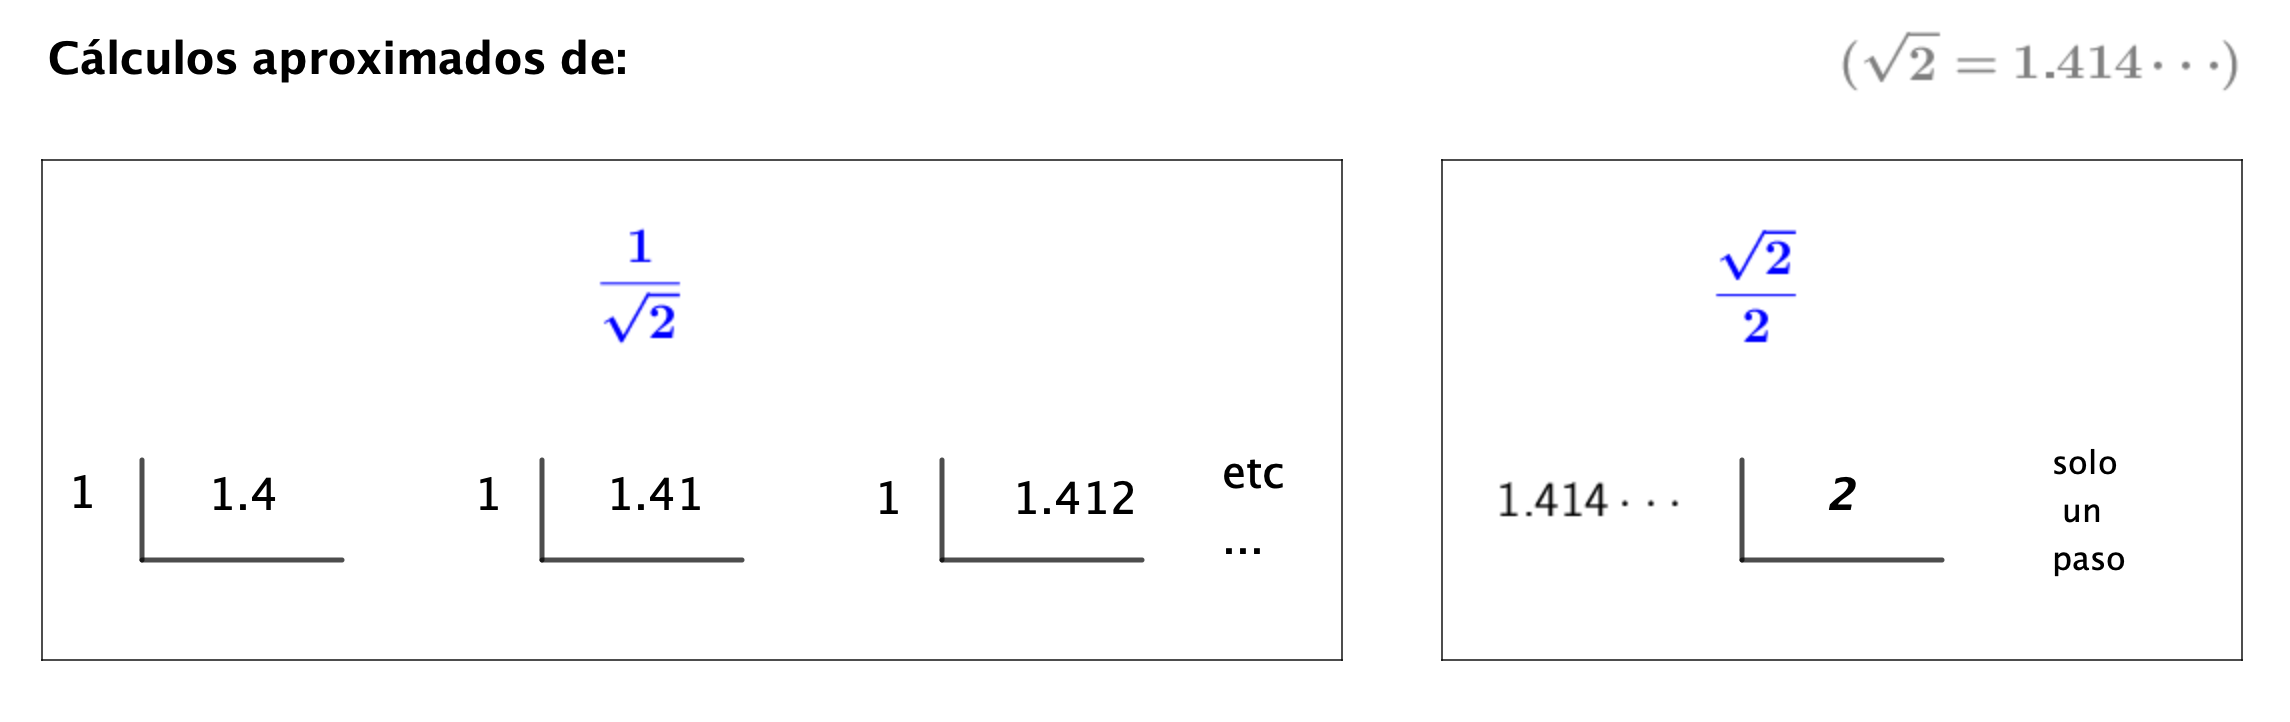
\includegraphics[width=.8\textwidth]{img-reales/reales19.png}
	\end{figure}

De todas formas, el proceso de racionalización es lo suficientemente importante para aprenderlos pues sus técnicas (multiplicar numerador y denominador por la expresión \emph{conjugada}) se usa en la simplificación de muchas expresiones algebraicas.

\vspace{5mm}
$\triangleright\quad$ Expresiones con solo un radical en el denominador:  hay que multiplicar y dividir por la cantidad adecuada para que el denominador se convierta en una expresión del tipo $\ \sqrt[n]{a^n}=a$ 

\begin{miejemplo}

\begin{small}
$\boldsymbol{ \dfrac{3}{2\sqrt{5}} }	\ = \dfrac{3}{2\sqrt{5}}\dfrac{\sqrt{5}}{\sqrt{5}}=\dfrac{3\sqrt{5}}{2(\sqrt{5})^2}=\ \boldsymbol{\dfrac{3\sqrt{5}}{10}}$
$;\qquad \ \ $
$\boldsymbol{ \dfrac{2}{ \sqrt[5]{25} } } = \  \dfrac{2}{ \sqrt[5]{5^2} } = \dfrac{2}{ \sqrt[5]{5^2} } \dfrac{\sqrt[5]{5^3}}{\sqrt[5]{5^3}}=\dfrac{2\sqrt[3]{5^3}}{\sqrt[3]{5^5}} =\ \boldsymbol{ \dfrac{2\sqrt[3]{5^3}}{5} }$\end{small}
\end{miejemplo}

\vspace{5mm}
$\triangleright\quad$ \normalsize{Expresiones} con suma o resta de dos raíces cuadradas en el denominador: se multiplicará y dividirá la fracción por la \emph{expresión conjugada} del denominador (el conjugado de una suma es una resta y viceversa). Se consigue así tener el producto de una suma por diferencia en el denominador que, al ser una diferencia de cuadrados, elimina las raíces cuadradas.

\begin{miejemplo}

\begin{small}$\boldsymbol{\dfrac{2}{2\sqrt{2}-\sqrt{5}}}\ = \dfrac{2}{2\sqrt{2}-\sqrt{5}}\,  \dfrac{2\sqrt{2}+\sqrt{5}}{2\sqrt{2}+\sqrt{5}} = \dfrac{2(2\sqrt{2}+\sqrt{5})}{(2\sqrt{2})^2-(\sqrt{5})^2}=\dfrac{2(2\sqrt{2}+\sqrt{5})}{2^2\cdot 2-5} \ = \boldsymbol{\dfrac{4\sqrt{2}+2\sqrt{5}}{3}}$	\end{small}
\end{miejemplo}
\vspace{5mm}

\begin{myexampleblock}{Raíz de \emph{Ramanujan}}

\begin{figure}[H]
	\centering
	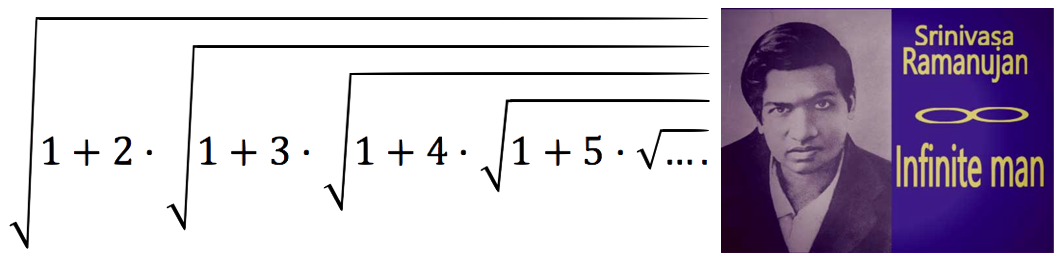
\includegraphics[width=1\textwidth]{img-reales/reales17.png}
	\end{figure}

\vspace{2mm}
\begin{multicols}{2}
	
	$3=\sqrt{9}$
	
	$=\sqrt{1+8}=$
	
	$=\sqrt{1+2\cdot 4}=$
	
	$=\sqrt{1+2\sqrt{16}}=$
	
	$=\sqrt{1+2\sqrt{1+15}}=$
	
	$=\sqrt{1+2\sqrt{1+3\cdot 5}}=$
	
	$=\sqrt{1+2\sqrt{1+3\sqrt{25}}}=$
	
	$=\sqrt{1+2\sqrt{1+3\sqrt{1+4\cdot 6}}}=$
	
	$=\sqrt{1+2\sqrt{1+3\sqrt{1+4\sqrt{36}}}}=$
	
	$=\sqrt{1+2\sqrt{1+3\sqrt{1+4\sqrt{1+\cdots}}}}$

\end{multicols}

\vspace{2mm}
Srinivasa Ramanujan Iyengar o simplemente como Ramanujan (1887-1920), fue un matemático autodidacta indio que, con una mínima educación académica en matemáticas puras, hizo contribuciones extraordinarias al análisis matemático, la teoría de números, las series y las fracciones continuas. Ramanujan desarrolló inicialmente su propia investigación matemática en forma aislada, que fue rápidamente reconocida por los matemáticos indios. Cuando sus habilidades se hicieron evidentes para una comunidad matemática más amplia, centrada en Europa en ese momento, comenzó su famosa colaboración con el matemático británico G. H. Hardy. Redescubrió teoremas conocidos previamente, además de formular numerosas nuevas proposiciones.

\vspace{2mm}

El número $1729$ se conoce como el número de Hardy-Ramanujan por una famosa anécdota del matemático británico G. H. Hardy en relación con una visita al hospital para ver a Ramanujan. En palabras de Hardy: ``Recuerdo una vez que fui a verle cuando estaba enfermo en Putney. Había viajado en el taxi número $1729$ y mencioné que me parecía un número poco notable, y que esperaba que esto no fuera un mal presagio. ``!No!'', me respondió, ``!`es un número muy interesante!; es el número más pequeño expresable como la suma de dos cubos de dos maneras diferentes''. En efecto, la cifra tiene dos descomposiciones diferentes: $9^3+{10}^3=1^3+{12}^3=1729$

\vspace{2mm}

\begin{center} \rule{250pt}{0.1pt} \end{center}

\vspace{2mm}

\color{teal}
\textsf{\begin{small}`El hombre que conocía el infinito'  es una película británica biográfica sobre Ramanujan, del director Matthew Brown, estrenada en $2015$. El actor Dev Patel representa a Srinivasa Ramanujan, un matemático hindú que después de crecer en la pobreza en Madrás, India, es admitido a regañadientes en la exclusiva Universidad de Cambridge en el periodo previo a la Primera Guerra Mundial, donde después de salvar situaciones con matemáticos ingleses muy conservadores que al principio no le hacen la vida fácil, reconocen su genio, es elegido miembro de la Sociedad Matemática de Londres y es reconocido como un pionero en teorías matemáticas formuladas guiado por su profesor, G. H. Hardy.\end{small}\normalsize{.}}


\end{myexampleblock}

\color{black}
\vspace{5mm}
\begin{miejercicio}

$\boldsymbol{ \dfrac{1+\sqrt{x}}{1-\sqrt{x}} } \ = 	\dfrac{1+\sqrt{x}}{1-\sqrt{x}}\,  \dfrac{1+\sqrt{x}}{1+\sqrt{x}}=\dfrac{(1+\sqrt{x})^2}{1^2-(\sqrt{x})^2}=\dfrac{1+2\sqrt{x}+x}{1-x} = \ \boldsymbol{\dfrac{1+x+2\sqrt{x}}{1-x}}$
\end{miejercicio}

\begin{miejercicio}

$\boldsymbol{ \dfrac{2}{\sqrt{3}-\sqrt{5}+2\sqrt{7}} } \ = 
\dfrac{2}{(\sqrt{3}-\sqrt{5})+2\sqrt{7}}=
\dfrac{2}{(\sqrt{3}-\sqrt{5})+2\sqrt{7}}\, \dfrac{(\sqrt{3}-\sqrt{5})-2\sqrt{7}}{(\sqrt{3}-\sqrt{5})-2\sqrt{7}}=$

$= \dfrac{2[(\sqrt{3}-\sqrt{5})-2\sqrt{7}]}{(\sqrt{3}-\sqrt{5})^2-(2\sqrt{7})^2}=
 \dfrac{2[\sqrt{3}-\sqrt{5}-2\sqrt{7}]}{3-2\sqrt{15} +5-2^2\cdot 7}=
\dfrac{2[\sqrt{3}-\sqrt{5}-2\sqrt{7}]}{-20-2\sqrt{15} }=  
$

$=\dfrac{\sqrt{3}-\sqrt{5}-2\sqrt{7}}{-10-\sqrt{15} }= \dfrac{-\sqrt{3}+\sqrt{5}+2\sqrt{7}}{10+\sqrt{15} } \, \dfrac{10-\sqrt{15}}{10-\sqrt{15}}= 
\dfrac{(10+\sqrt{15})(-\sqrt{3}+\sqrt{5}+2\sqrt{7})}{10^2-(\sqrt{15})^2 }=$

$=\ \boldsymbol{
\dfrac{(10+\sqrt{15})(-\sqrt{3}+\sqrt{5}+2\sqrt{7})}{85 } }
\quad $ \begin{footnotesize}
 (faltaría multiplicar el numerador)	
 \end{footnotesize}

\end{miejercicio}

\vspace{10mm}

\begin{myalertblock}{ Racionalizaciones más complejas (ampliación)}
	
\begin{multicols}{3}
Denominador

$\quad \sqrt[n]{a}$

$\quad \sqrt{a} \pm \sqrt{b}$

$\quad \sqrt[3]{a} \pm \sqrt[3]{b}$

Factor racionalizante

$\quad \sqrt[n]{a^{n-m}}$ 

$\quad \sqrt{a} \mp \sqrt{b}$

$\quad \sqrt[3]{a^2} \mp \sqrt[3]{ab} + \sqrt[3]{b^2}$

Denominador racionalizado

$\qquad \qquad a$

$\qquad \qquad a-b$

$\qquad \qquad a\pm b$
	
\end{multicols}




\textcolor{gris}{En la última fila hemos usado que $\ \ (x\pm y)\cdot(x^2\mp xy+y^2) \ = \ x^3\pm y^3$ y hemos sustituido $x$ e $y $ por $\sqrt[3]{a}$ y  $\sqrt[3]{b}$, respectivamente.}

\vspace{2mm} En general:

$$(\sqrt[n]{a}-\sqrt[n]{b})\cdot (\sqrt[n]{a^{n-1}}+\sqrt[n]{a^{n-2}b}+\cdots + \sqrt[n]{b})=a-b $$

$$(\sqrt[n]{a}+\sqrt[n]{b})\cdot (\sqrt[n]{a^{n-1}}-\sqrt[n]{a^{n-2}b}+\cdots + \sqrt[n]{b}) \ = \ \begin{cases}\  a+b& n \text{ impar} \\ \  a-b& n \text{ par} \end{cases}$$

Un factor es el factor racionalizante del otro.

\vspace{2mm}\underline{ejemplos}: 

\vspace{2mm} \begin{small}$\dfrac{2}{\sqrt[3]{4}-\sqrt[3]{2}}=\dfrac{2}{\sqrt[3]{4}-\sqrt[3]{2}}\cdot \dfrac{\sqrt[3]{4^2}+\sqrt[3]{4\cdot 2}+\sqrt[3]{2^2}}{\sqrt[3]{16}+\sqrt[3]{8}+\sqrt[3]{4}}=\dfrac{2(\sqrt[3]{16}+\sqrt[3]{8}+\sqrt[3]{4})}{(\sqrt[3]{4})^3-(\sqrt[3]{2})^3}=\dfrac{\cancel{2} ((\sqrt[3]{16}+\sqrt[3]{8}+\sqrt[3]{4})}{\cancel{2}}$\end{small}




\vspace{2mm} $\dfrac{1}{\sqrt[5]{2}-1}=\dfrac{1}{\sqrt[5]{2}-1} \cdot \dfrac{\sqrt[5]{2^4}+\sqrt[5]{2^3}+\sqrt[5]{2^2}+\sqrt[5]{2}+1}{\sqrt[5]{2^4}+\sqrt[5]{2^3}+\sqrt[5]{2^2}+\sqrt[5]{2}+1} = \dfrac{\sqrt[5]{2^4}+\sqrt[5]{2^3}+\sqrt[5]{2^2}+\sqrt[5]{2}+1}{(\sqrt[5]{2})^5-1}=\sqrt[5]{16}+\sqrt[5]{8}+\sqrt[5]{4}+\sqrt[5]{2}+1$	

\vspace{2mm} $\dfrac{1}{\sqrt[3]{4}-\sqrt[3]{2}+1}=\dfrac{1}{\sqrt[3]{4}-\sqrt[3]{2}+\sqrt[3]{1}} \cdot \dfrac{{\sqrt[3]{2}+1}}{{\sqrt[3]{2}+1}}= \dfrac{\sqrt[3]{2}+1}{(\sqrt[3]{2})^3-(\sqrt[3]{1})^3}=\sqrt[3]{2}+1$
	
\vspace{5mm} \begin{large} \underline{Radicales dobles}:\end{large}

\vspace{2mm} $\boxed{ \subrayado{ \ \boldsymbol{ \sqrt{a \pm \sqrt{b}}\ = \ \sqrt{\dfrac{a+c}{2}} \pm \sqrt{\dfrac{a-c}{2}} } \  }  } \, ;\qquad a,b>0$

\color{gris}
\vspace{4mm}\underline{demostración}:

\vspace{2mm} llamando $\ \sqrt{a+\sqrt{b}}=\sqrt{x}+\sqrt{y} \ \text{ y } \ \sqrt{a-\sqrt{b}}=\sqrt{x}-\sqrt{y}$,

\vspace{2mm} sumando $\ \sqrt{a+\sqrt{b}}+ \sqrt{a-\sqrt{b}}=2\sqrt{x}$

\vspace{2mm} elevando al cuadrado $\ a+\cancel{\sqrt{b}}+a-\cancel{\sqrt{b}}+2\sqrt{a^2-b}=4x \ \to \ x=\dfrac{a+\sqrt{a^2-b}}{2}$

\vspace{2mm} \emph{condición}: $\ a^2-b=c^2\, , \ $ cuadrado perfecto!

\vspace{2mm} restando $\ \sqrt{a+\sqrt{b}}- \sqrt{a-\sqrt{b}}=2\sqrt{y} $

\vspace{2mm} y por el mismo procedimiento $ y=\dfrac{a-\sqrt{a^2-b}}{2}$

\vspace{2mm} con lo que $\ \sqrt{a \pm \sqrt{b}}\ = \ \sqrt{\dfrac{a+c}{2}} \pm \sqrt{\dfrac{a-c}{2}}\, \ \text{ con } \ c=\sqrt{a^2-b} $ \QED

\color{black}
\vspace{2mm}\underline{ejemplos}: 

\vspace{2mm} $\sqrt{7+\sqrt{40}}=\left[\mqty{a=7\\b=40} \  \right| \left. \ c=\sqrt{7^2-40}=3 \right] = \sqrt{\dfrac{7+3}{2}}+\sqrt{\dfrac{7-3}{2}}=\sqrt{5}+\sqrt{2}$

\vspace{2mm}  $\sqrt{12-\sqrt{108}}=\left[\mqty{a=12\\b=102} \  \right| \left. \ c=\sqrt{12^2-108}=6 \right] = \sqrt{\dfrac{12+6}{2}}-\sqrt{\dfrac{12-6}{2}}=3-\sqrt{3}$


\vspace{5mm} $\boxed{ \subrayado{ \ \boldsymbol{ 
\sqrt{S\pm 2\sqrt{P}} \ = \ \sqrt{a}  \pm \sqrt{b}
} \ } } \, ;\qquad a,b>0;\quad S=a+b;\ P=a\cdot b$

\color{gris}
\vspace{4mm}\underline{demostración}:

\vspace{2mm} $(\sqrt{a}\pm \sqrt{b})^2=a+b\pm 2\sqrt{ab}=S\pm 2\sqrt{P}\, ; \quad S=a+b;\ P=a\cdot b$

\vspace{2mm} \normalsize{sacando} raíz cuadrada $\ |\sqrt{a} \pm \sqrt{b}| = \sqrt{S\pm 2\sqrt{P}}$

\color{black}
\vspace{2mm}\underline{ejemplos}: 

\vspace{2mm} $\sqrt{9+\sqrt{80}}=\sqrt{9+2\sqrt{20}} =
\left[ \mqty{S=9\\P=20} \ \right| \left. \  \mqty{a=5\\b=4} \right]=\sqrt{5}+\sqrt{4}=\sqrt{5}+2$

\vspace{2mm} $\sqrt{7-\sqrt{48}}=\sqrt{7-2\sqrt{12}} =
\left[ \mqty{S=7\\P=12} \ \right| \left. \  \mqty{a=4\\b=3} \right]=\sqrt{4}-\sqrt{3}=2-\sqrt{3}$

\color{gris}

\vspace{4mm}Como ejercicio, probar que:

\vspace{2mm} $\qquad \sqrt{\sqrt{38+12\sqrt{2}} + \sqrt{26-8\sqrt{3}}+1}= \ \cdots \ = \sqrt{6}+1$

\vspace{2mm} $\qquad \sqrt{9+2\sqrt{7+6\sqrt{6+4\sqrt{2}}}}= \ \cdots \ = 3+\sqrt{2}$
\color{black}	
\end{myalertblock}

\vspace{5mm}
\begin{figure}[H]
	\centering
	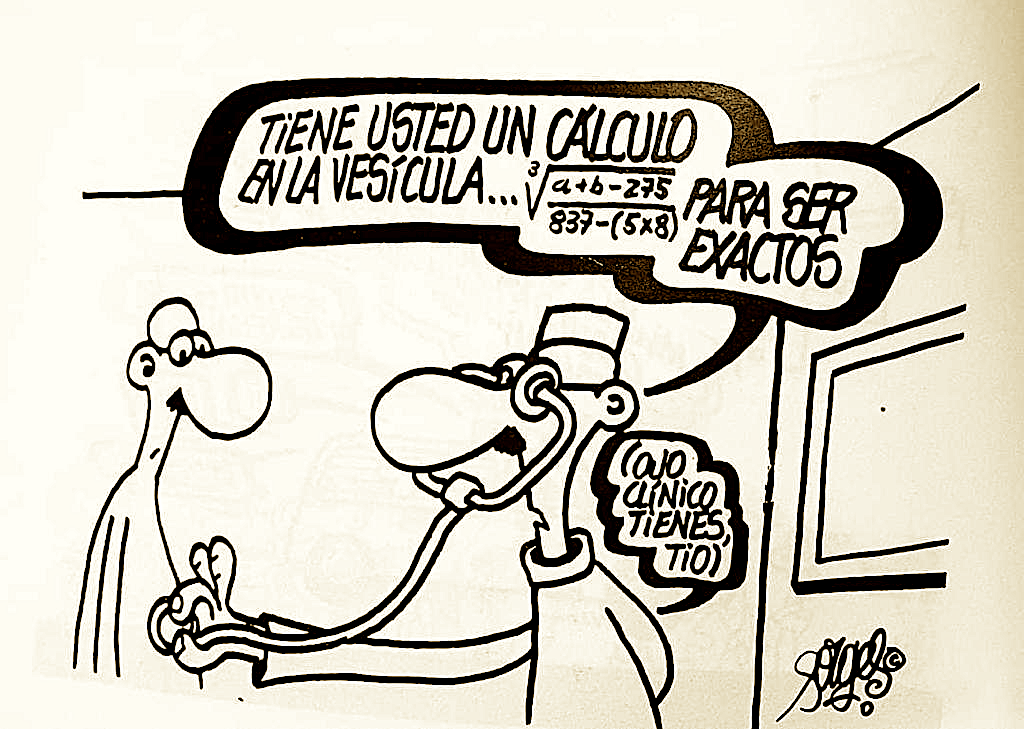
\includegraphics[width=.75\textwidth]{img-reales/reales21.png}
	\end{figure}

\vspace{1cm}
\section{Logaritmos}

\begin{tikzpicture}
	\fill [left color=red!50, right color=teal!50] (0,0) rectangle (3.5,.1);
	\fill [left color=teal!50, right color=blue!50] (3.5,0) rectangle (7.5,.1);
	\end{tikzpicture}
\vspace{0.5cm}


\begin{myexampleblock}{Escala logarítmica y órdenes de magnitud}
	
La utilidad fundamental de los logaritmos radica en manejar `escalas logarítmicas’. 

\vspace{2mm} Una escala logarítmica es una escala de medida que utiliza el logaritmo de una cantidad física en lugar de la propia cantidad.

\vspace{2mm} Un ejemplo sencillo de escala logarítmica muestra divisiones igualmente espaciadas en el eje vertical de un gráfico marcadas con 1, 10, 100, 1000, …, en vez de 0, 1, 2, 3, …

\vspace{2mm} La presentación de datos en una escala logarítmica es muy útil cuando los datos cubren una amplia gama de valores - el logaritmo los reduce a un rango más manejable.

\vspace{2mm} Ejemplos de escalas logarítmicas son:

--- Cuando hablamos del PH , que es una concentración media según una escala logarítmica.

--- Cuando medimos la intensidad de los terremotos de acuerdo a la escala Richter.

--- Cuando hablamos del brillo de las estrellas (magnitud aparente).

--- La intensidad del sonido (Decibelios) también es una escala logarítmica.

\vspace{2mm}
Se basan en órdenes de magnitud, en lugar de una escala lineal estándar. El valor de cada marca de la escala es 10 veces la marca anterior (logaritmos decimales). Se utilizan órdenes de magnitud para hacer comparaciones aproximadas. Si los números difieren en un orden de magnitud, x es aproximadamente diez veces diferente en cantidad que y . Si los valores difieren en dos órdenes de magnitud, difieren en un factor de aproximadamente 100. Dos números del mismo orden de magnitud tienen aproximadamente la misma escala: el valor mayor es menos de diez veces el valor menor.

\underline{Escala logarítmica}

\begin{multicols}{2}
$\quad$

La imagen muestra cómo podría realizarse un mapa a escala logarítmica de todo el Universo visible, de manera que -al igual que ocurre con los mapas terrestres- preserve a pequeña escala las formas, mostrando a la vez todo el rango de distancias astronómicas (desde el espacio local, cercano a la Tierra, hasta los objetos situados a escala cosmológica como los quasars).
\begin{figure}[H]
	\centering
	\includegraphics[width=0.4\textwidth]{img-reales/reales12.png}
	\end{figure}
\end{multicols}

\underline{Órdenes de magnitud}
\begin{figure}[H]
	\centering
	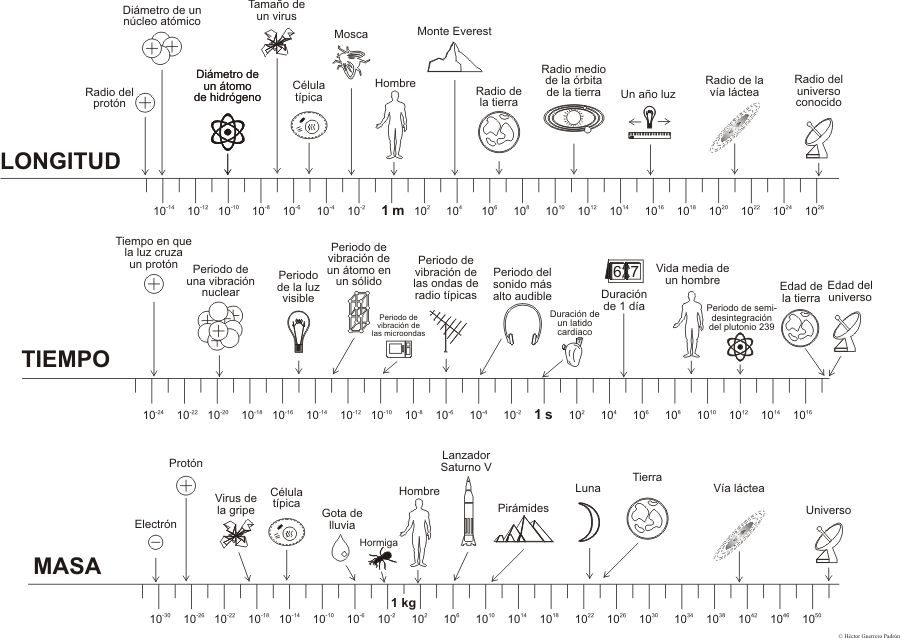
\includegraphics[width=1\textwidth]{img-reales/reales14.png}
	\end{figure}

\end{myexampleblock}

\color{teal}
\rule{250pt}{0.1pt}	

A partir del siglo XVI, los cálculos que se precisaban hacer, debido principalmente a la expansión comercial y al perfeccionamiento de las técnicas de navegación, eran de tal magnitud que surgía la necesidad de encontrar algoritmos que los facilitasen. 

\vspace{3mm} Los logaritmos fueron introducidos por John Napier a principios del siglo XVII como un medio de simplificación de los cálculos y fueron prontamente adoptados por científicos, ingenieros, banqueros y otros para realizar operaciones fácil y rápidamente. Los logaritmos permitían transformar los productos en sumas y los cocientes en restas con lo que la facilidad del cálculo quedaba garantizada. Aún más, los logaritmos transformas potencias (y raíces) en meros productos por el exponente. 

\vspace{3mm} Hoy día, su utilidad radica en la sencillez que proporciona su uso en muchas expresiones simbólicas y en el uso de escalas logarítmicas.

\begin{center}
\rule{200pt}{0.1pt}	
\end{center}

\vspace{-3mm} En ciencia se acostumbra a trabajar con números muy grandes: 

\hspace{5mm} --- Masa del Sol, $M_{\sun}= 1984000000000000000000000000000000\, $ kg.

\hspace{5mm} --- Masa del electrón, $m_{e^{-}}=0.000000000000000000000000000000911\, $ kg. 

\vspace{2mm} Para esto se usa la \underline{\emph{notación científica}}, $\boldsymbol{m \times 10^e}$; $m\in [1,10[ $ es la mantisa y $e$ el exponente de base 10. Así,
$\ 243000000000=2.43\times 10^{11} \, ; \qquad 0.000008724=8.274\time 10^{-6}$

\vspace{-5mm}
\begin{flushright}
\rule{250pt}{0.1pt}	
\end{flushright}
\color{black}
\vspace{5mm}


\begin{definition}[ Logaritmos]

\begin{multicols}{2}
Sea $\ a>0\, , \ a\neq 1\, , \ $  	llamamos \emph{logaritmo} en base $ \ a \ $ de un número $ \ P \ $ , y lo denotamos por $\ \log_aP \, , \ $ al número al que hay que elevar $\ a \ $ para obtener $\ P \, . $

$$
\boxed{ \ \boldsymbol{
\log_a P \ = \ b \ \leftrightarrow \ a^P\ = \ b
} \ }
$$

$\quad$
\begin{figure}[H]
	\centering
	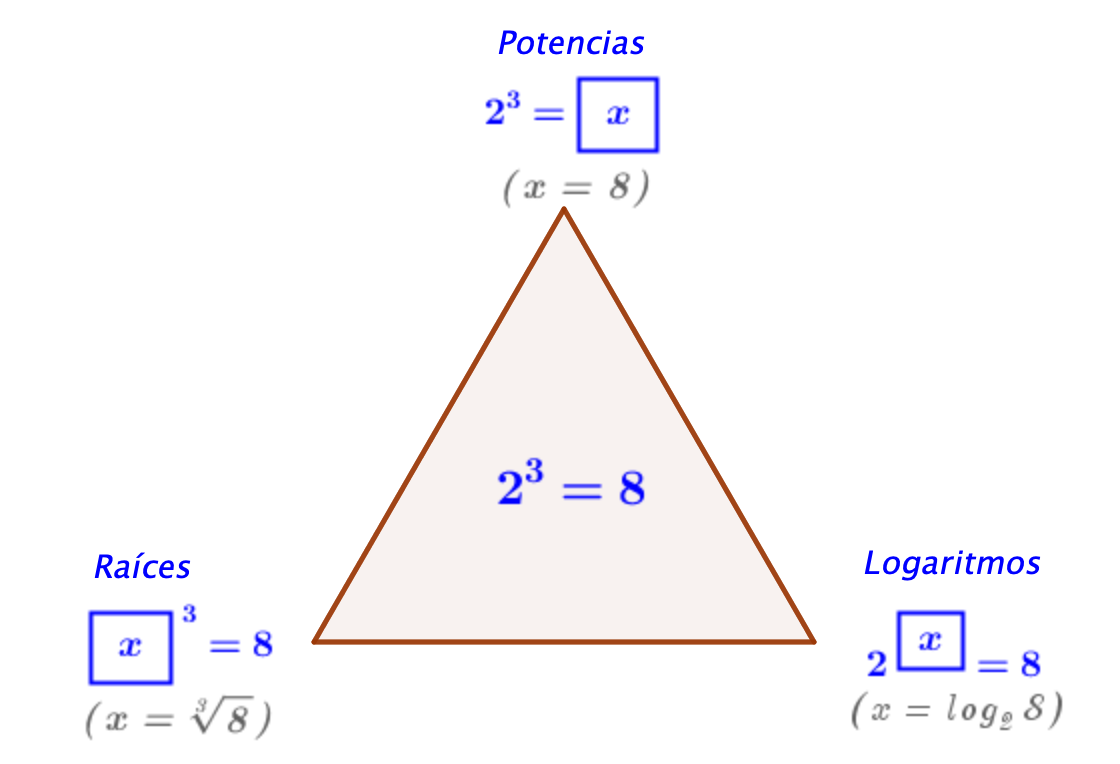
\includegraphics[width=0.5\textwidth]{img-reales/reales13.png}
	\end{figure}
\end{multicols}
\end{definition}


\begin{miejemplo}

$\log_28=3 \leftrightarrow 2^3=8;\quad \log_525=2 \leftrightarrow 5^2=25;\quad \log_{10}0.0001 =-4 \leftrightarrow 10^{-4}=0.0001$	
\end{miejemplo}

\vspace{5mm}

\begin{theorem}[ Propiedades de los logaritmos]
	
	\begin{enumerate}[P1. ]
	\item $\boldsymbol{ \log_aa=1}$
	
	\textcolor{gris}{$\log_aa=b \ \leftrightarrow \ a^b=1 \ \to \ b=1$ \QED} 	
	
	\item $\boldsymbol{\log_a1=0}$
	
	\textcolor{gris}{$\log_a1=b \ \leftrightarrow \ a^b=1 \ \to \ b=0$ \QED} 	
	
	\item $\boldsymbol{\log_a (A\cdot B)\ = \ \log_aA\ + \ \log_aB }\quad $ El log. del producto la suma de log.

\color{gris}
	\small{	
	$\begin{cases}
	\ \log_a(A\cdot B)=b \ \leftrightarrow \ a^b=A\cdot B \\
	\ \log_aA=b_1 \ \leftrightarrow \ a^{b_1}=A	\\
	\ \log_aB=b_2 \ \leftrightarrow \ a^{b_2}=B
	\end{cases}
	a^b=A\cdot B=a^{b_1}a^{b_2}=a^{b_1+b_2} \ \to \ b=b_1+b_2 $ \QED }	
	\color{black} 
	
	\item $\boldsymbol{\log_a \left(\dfrac A B \right)\ = \ \log_aA\ - \ \log_aB }\quad $ El log. del cociente la resta de log\normalsize{.}
	
	\color{gris}
	\small{	
	$\begin{cases}
	\ \log_a(A/ B)=b \ \leftrightarrow \ a^b=A/B \\
	\ \log_aA=b_1 \ \leftrightarrow \ a^{b_1}=A	\\
	\ \log_aB=b_2 \ \leftrightarrow \ a^{b_2}=B
	\end{cases}
	a^b=A/ B=a^{b_1}/a^{b_2}=a^{b_1-b_2} \ \to \ b=b_1-b_2 $ \QED }	
	\color{black} 
	
	\item $\boldsymbol{\log_a (A^n)\ = \ n\cdot \log_aA} \quad $ \small{El log. de una potencia es el exponente por el log de la base}\normalsize{.}
	
	\color{gris}{
		\small{	
	$\begin{cases}
	\ \log_a(A^n)=b \ \leftrightarrow \ a^b=A^n \\
	\ \log_aA=b_1 \ \leftrightarrow \ a^{b_1}=A	\\
	\end{cases}
	a^b=A^n=(a^{b_1})^n=a^{n\, b_1}\ \to \ b=n\, b_1 $ \QED }	}
	\color{black} 

\end{enumerate}

\end{theorem}

De la última propiedad deducimos que el logaritmo de una raíz es el logaritmo del radicando dividido por el índice de la raíz:
$\quad \boldsymbol{ \log_a \sqrt[n]{A} }\ = \log_a A^{1/n} = \ (P5) \ = \frac 1 n \, \log_a A=\ \boldsymbol{ \dfrac{\log_aA}{n} }$ 


\begin{figure}[H]
	\centering
	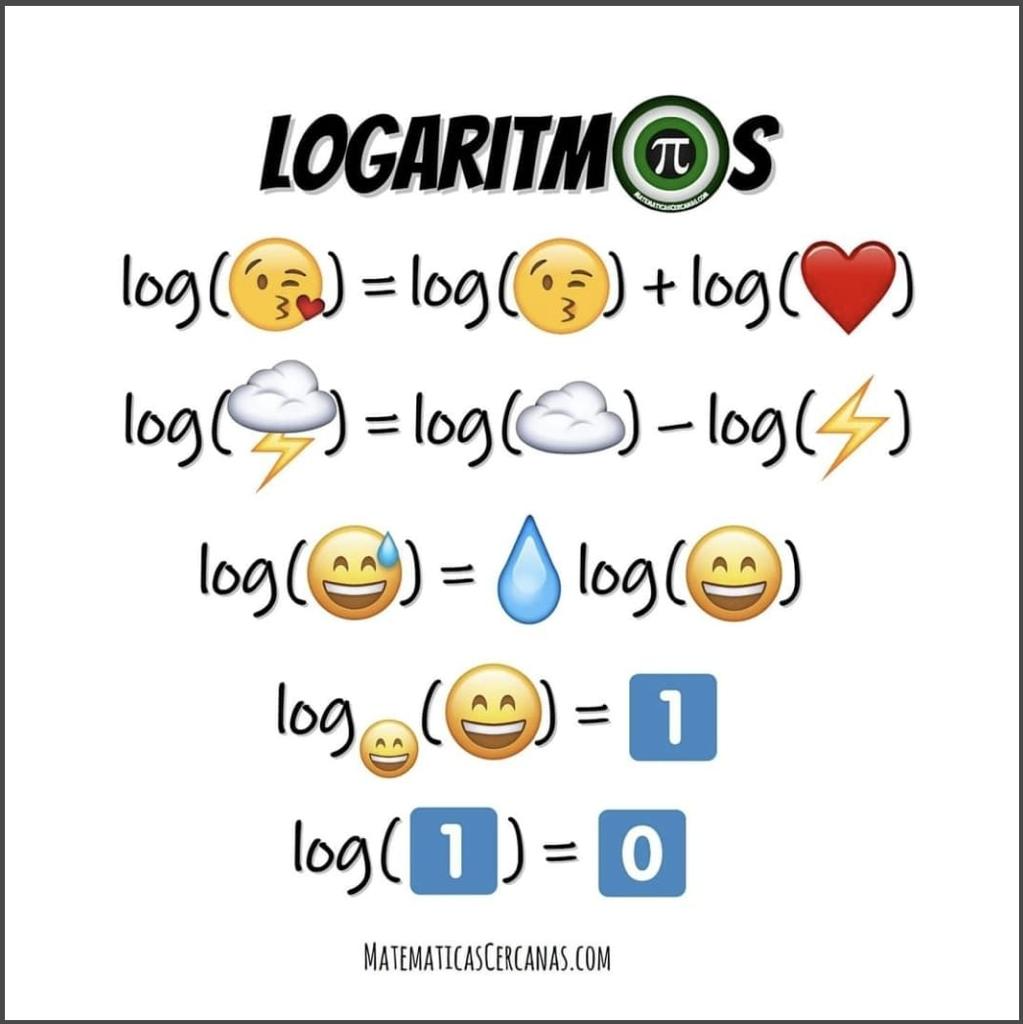
\includegraphics[width=0.4\textwidth]{img-reales/reales20.png}
	\end{figure}


\vspace{5mm}

\begin{theorem}[ Cambio de base en logaritmos]
	
	$$\boxed{\ \boldsymbol{ \log_aP\ = \ \dfrac{\log_c P}{\log_c a} } \ \ }$$
\end{theorem}

\underline{Demostración} 

$\log_aP=b\ \leftrightarrow \ a^b=P\, ,  $ tomemos logaritmos en otra base, $ \ c\ $ por ejemplo:

$\log_c (a^b) = \log_c P \, $ aplicando la propiedad P5 de los logaritmos,

$b\, \log_c a = \log_c P \ \to \ b=\dfrac{\log_c P}{\log_c a} \, $ pero $\ b=\log_aP\, , \  $ luego

$\log_aP\ = \ \dfrac{\log_c P}{\log_c a}$ \QED

\vspace{5mm}

Como $\log_aP=b \leftrightarrow P=a^b>0$, un número positivo $a$ elevado a cualquier número $b$ siempre es positivo, \emph{el logaritmo solo se puede calcular para número estrictamente positivos} (el dominio de la función logarítmica es $\mathbb R^+$). Al poder ser $b$ cualquier número real, \emph{el logaritmo de un número positivo puede ser cualquier número real, positivo, negativo o nulo} (el recorrido de la función logarítimca es $\mathbb R$). 

\vspace{5mm}

Con una sola base que tuviésemos de logaritmos sería más que suficiente. En las calculadoras aparecen los logaritmos más usuales que son los \emph{logaritmos decimales}, de base $10$, y los \emph{logaritmos neperianos} o \emph{naturales} cuya base es el número $\ e\,\approx \, 2.7182\cdots\,  $. 
Sus representaciones son: 
$\qquad \log_{10} \ \equiv \ \boldsymbol{ Log} \, ; \qquad  \log_e\ \equiv \boldsymbol{ \ln}$


\vspace{5mm}

\begin{adjustwidth}{100pt}{100pt}
\begin{cuadro-naranja}
$$\boldsymbol{ \log_a a^x\ = \ x \qquad 	 \qquad  \qquad  a^{\log_a x}\ = \ x }$$

\vspace{1mm}
\end{cuadro-naranja}
\end{adjustwidth}

\color{gris}
\underline{Demostracines}:

$\log_a^x=x\cancelto{1}{\log_a a}=x$ \QED

$a^{\log_a x}=P\ $ tomamos logaritmos, $\ \log_a{a^{\log_a x}}=\log_a P;\ \ \log_a x\cdot \cancelto{1}{\log_a a}=\log_a P \ \to \ x=P$ \QED
\color{black}

\vspace{5mm}
\begin{miejercicio}

Calcula los siguientes logaritmos aplicando la definición:

\vspace{2mm} $\log_2 1024; \qquad \log_2 0.5;\qquad \log_5 125;\qquad	 \log_{\frac 1 3}\frac 1 9;\qquad \log_4 \sqrt{2}$

\rule{300pt}{0.1pt}

$\triangleright \quad \log_2 1024=x \ \leftrightarrow \ 2^x=1024=2^{10} \ \to \ x= \ \boldsymbol{ \log_2 1024=10 }$

\vspace{2mm} $\triangleright \quad \log_2 0.5=x \ \leftrightarrow \ 2^x=0.5=\frac 1 2 =2^{-1} \ \to \ x=\ \boldsymbol{\log_2 0.5=-1}$

\vspace{2mm} $\triangleright \quad \log_5 125=x \ \leftrightarrow \ 5^x=125=5^3 \ \to \ x=\ \boldsymbol{\log_5 125=3}$

\vspace{2mm} $\triangleright \quad \log_{\frac 1 3} \frac 1 9 = x \ \leftrightarrow \ \left( \frac 1 3 \right)^x=\frac 1 9 = \left( \frac 1 3 \right)^2 \ \to \ x=\ \boldsymbol {\log_{\frac 1 3} \frac 1 9 = 2}$

\vspace{2mm} $\triangleright \quad \log_4 \sqrt{2}=x \ \leftrightarrow \ 4^x=\sqrt{2} \ \to {(2^2)}^x=2^{\frac 1 2 } \ \to \ 2x=\frac 1 2 \ \to \ x=\ \boldsymbol{\log_4 \sqrt{x}=\frac 1 4}$
\end{miejercicio}


\begin{miejercicio}

Encuentra la base de los siguientes logaritmos:

\vspace{2mm} $\log_a 243=5;\qquad \log_a 0.125=3;\qquad \log_a 0.001=-3;\qquad \log_a 3=2;\qquad \log_a \sqrt[4]{5}=\frac 1 2 $	

\rule{300pt}{0.1pt}

$\log_a 243=5 \ \leftrightarrow \ a^5=243=3^5 \ \to \boldsymbol{ a}= \sqrt[5]{243} =\boldsymbol{ 5}$

\vspace{2mm} $\log_a 0.125=3 \ \leftrightarrow \ a^3=0.125=\frac 1 8 =2^{-3}=\left( \frac 1 2 \right)^3 \ \to \ \boldsymbol{a}=\sqrt[3]{125}=\boldsymbol{ \frac 1 2}$

\vspace{2mm} $\log_a 0.001=-3 \ \leftrightarrow \ a^{-3}=0.001=10^{-3} \ \to \ \boldsymbol{a}= 0.001^{-1/3}= \frac 1 {\sqrt[3]{0.001}}=\boldsymbol {10}$

\vspace{2mm} $\log_a 3=2 \ \leftrightarrow \ a^2=3 \ \to \ a^2=(\sqrt{3})^2 \ \to \ \boldsymbol{a}=\sqrt{3} =\boldsymbol{\sqrt{3}}$
\end{miejercicio}

\begin{miejercicio}

Calcula: $\qquad 3^{1/x}=9;\qquad \log_{16}0.5=x;\qquad \log_{10}0.00001=x;\qquad log_x 125=\frac 32$	


\rule{300pt}{0.1pt}

$3^{1/x}=9=3^2 \ \to \ \frac 1 x = 2 \ \to \ 1=2x \ \to \ \boldsymbol{x=\frac 1 2} $

\vspace{2mm} $\log_{16}0.5=x \ \leftrightarrow \ 16^x=0.5=\frac 1 2 \ \to \ (2^4)^x=2^{4x}=2^{-1} \ \to \ 4x=-1 \ \to \ \boldsymbol{x=-\frac 1 4}$

\vspace{2mm} $\log_{10}0.00001=x \ \leftrightarrow \ 10^x=0.00001=10^{-5} \ \to \ \boldsymbol{x=-5}$

\vspace{2mm} $log_x 125=\frac 32 \ \leftrightarrow \ x^{3/2}=125=5^3 \ \to \ \boldsymbol{x}=(x^{3/2})^{2/3}=(5^3)^{2/3}=5^2=\boldsymbol{25}$	
 \end{miejercicio}
 


\begin{miejercicio}

Calcula: $\qquad \log_3 1 +\log_2 64 +\log_3 9 + \log_7 49$	


\rule{300pt}{0.1pt}

$\log_3 1 +\log_2 64 +\log_3 9 + \log_7 49=\cancelto{0}{\log_3 1} +\log_2 2^6 +\log_3 3^2 + \log_7 7^2=0 +6 \cancelto{1}{\log_2 2} +2 \cancelto{1}{\log_3 3} + 2 \cancelto{1}{\log_7 7}=6+2+2=\boldsymbol{ 10}$

\end{miejercicio}


\begin{miejercicio}

Calcula $x:\qquad \ln x=\ln 3+\ln 2-\ln 6;\qquad \mathrm{Log}x	=3\mathrm{Log}2-\frac 1 4 \mathrm{Log}16$

\rule{300pt}{0.1pt}

$\triangleright \quad \ln x=\ln 3+\ln 2-\ln 6=\ln(3\cdot 2)-\ln 6=\ln\left( \dfrac {3\cdot 2}{6} \right)=\ln 1 \ \to \ \boldsymbol{x=1} $

\vspace{2mm} $\triangleright \quad \mathrm{Log}x	=3\mathrm{Log}2-\frac 1 4 \mathrm{Log}16 \ \to \ \mathrm{Log} x= \mathrm{Log}2^3-\mathrm{Log}16^{1/4}= \mathrm{Log} \left( \dfrac{2^3}{\sqrt[4]{16}} \right)=\mathrm{Log} \dfrac 8 2 = \mathrm{Log} 4 \ \to \ \boldsymbol{x=4}$

\end{miejercicio}


\begin{miejercicio}

Desarrolla la siguiente expresión usando las propiedades de los logaritmos.


\rule{300pt}{0.1pt}

\vspace{2mm} $\boldsymbol{ \ln \dfrac{a^2\sqrt[5]{b}}{\sqrt[3]{c^4}}} = \ln(a^2\sqrt[5]{b})-\ln\sqrt[3]{c^4}=\ln a^2 +\ln \sqrt[5]{b}-\ln\sqrt[3]{c^4}=\boldsymbol{ 2\ln a +\frac 1 5 \ln b - \frac 4 3 \ln c }$ 
	
\end{miejercicio}

\begin{miejercicio}

Comprime la expresión siguiente para que el logaritmos aparezca una sola vez.


\rule{300pt}{0.1pt}

\vspace{2mm} $\boldsymbol{3\mathrm{Log} x +\frac 12 \mathrm{Log} (1-x)}=\mathrm{Log} x^3  + \mathrm{Log}  \sqrt{1-x}= \mathrm{Log} \left( x^3\, \sqrt{1-x} \right)$
	
\end{miejercicio}


\vspace{1cm}
\section{Números combinatorios. Binomio de Newton}

\begin{tikzpicture}
	\fill [left color=red!50, right color=teal!50] (0,0) rectangle (3.5,.1);
	\fill [left color=teal!50, right color=blue!50] (3.5,0) rectangle (7.5,.1);
	\end{tikzpicture}
\vspace{0.5cm}

\begin{definition}[ Factorial de un número]
	
	Se llama factorial de un número natural, $n\in \mathbb N$, y se representa por $\boldsymbol{n!}$, al producto de los factores consecutivos que empiezan por la unidad y acaban en $n$:
	
	$$\boldsymbol{ n! \ = \ 1\cdot 2 \cdot 3 \cdot \cdots \cdot (n-2) \cdot (n-1)\cdot n } \ = \ \displaystyle \prod_{k=1}^n k \qquad \text{(productorio)}$$
	
Por convenio, $\ 0!=1\, ; \qquad $ Es evidente que $\ n!=n\cdot (n-1)!$
\end{definition}


\begin{definition}[ Número combinatorio]
	.Se define el \textbf{número combinatorio $\boldsymbol{n}$ sobre $\boldsymbol{k}$}, con $\boldsymbol{n,k \in \mathbb N \, \wedge \ k\le n}$, y se denota por $\boldsymbol{\mqty(n\\k)}$, como:
	
	\vspace{2mm} $$\boxed{\ \boldsymbol{ \mqty(n\\k) \ = \ \textcolor{gris}{C_n^r} \ = \ \dfrac {n!}{k! \cdot (n-k)!} }	 \ }$$
	
	\vspace{2mm} Indican las combinaciones, sin repetición, de $n$-elementos tomados de $k$ en $k$ o el número de subconjuntos de $k$-elementos de un conjunto de $n$-elementos.
\end{definition}

\begin{theorem}[ Propiedades de los números combinatorios]
	. Propiedades de los números combinatorios.
	
	\begin{small}
	$$\mqty(n\\r)=\mqty(n\\n-r); \qquad \mqty(n\\0)=\mqty(n\\n)=1; \qquad \mqty(n\\r)+\mqty(n\\r+1)=\mqty(n+1\\r+1)$$
	\end{small}	
\end{theorem}

\color{gris}
\begin{small}
\underline{demostraciones}:

\vspace{2mm} $\triangleright \quad \mqty(n\\n-r)=\dfrac{n!}{(n-r)![n-(n-r)]!}=\dfrac{n!}{(n-r)!\, r!}=\mqty(n\\r)\ $ \QED


\vspace{2mm} $\triangleright \quad \mqty(n\\0)=\dfrac{n!}{0! \, n!}=1;\qquad \mqty(n\\ n)=\dfrac{n!}{n!(n-n)!}=1\ $ \QED


\vspace{2mm} $\triangleright \quad  \mqty(n\\r)+\mqty(n\\r+1)=\dfrac{n!}{r!(n-r)!}+\dfrac{n!}{(r+1)!(n-r-1)!}= \dfrac{n!(r+1)}{(r+1)!(n-r)!}+\dfrac{n!(n-r)}{(r+1)!(n-r)!}=$

$= \dfrac{n![\cancel{r}+1+n-\cancel{r}]}{(r+1)(n-r)!}=\dfrac{n!(n+1)}{(r+1)![(n+1)-(r+1)!]}=\dfrac{(n+1)!}{(r+1)![(n+1)-(r+1)!]}=\mqty(n+1\\r+1)\ $ \QED

\end{small}

\color{black}

\vspace{5mm}
\begin{miejercicio}

Encuentra el valor de $x$ tal que $\ \mqty(x\\2)=3!$

\vspace{2mm} 
\rule{300pt}{0.1pt}

\vspace{2mm} $\mqty(x\\2)=\dfrac{x!}{2!\cdot (x-2)!}=\dfrac{x\cdot(x-1)\cdot\cancel{ (x-2)!}}{2\, \cancel{(x-2)!}}=\dfrac{x(x-1)}{2}=3!=6 \ \to $

\vspace{2mm} $\to \ x(x-1)=12 \ \to \ x^2-x-12=0 \ \to \begin{cases}
 \ x=-3 \notin \mathbb N \\ \ x\ =\ 4 \in \mathbb N	
 \end{cases} \ \text{ Sol.: } \ \boldsymbol{x=4}$	
\end{miejercicio}

\begin{miejercicio}

Resuelve: $\quad \dfrac{m!}{(m-1)!}=\mqty(m\\2)$
\vspace{2mm} 

\rule{300pt}{0.1pt}	

\vspace{2mm} Al tener $\ \mqty(m\\2) \ \to \ m\in \mathbb N\, , /\ m>2$

\vspace{2mm} $\dfrac{m!}{(m-1)!}= \dfrac{m\cdot \cancel{(m-1)!}}{\cancel{(m-1)!}}=m $

$\mqty(m\\2)=\dfrac{m!}{2!\cdot (m-2)!}=\dfrac{m\cdot (m-1) \cdot \cancel{(m-2)!}}{2\cdot \cancel{(m-2)!}}=\dfrac{m(m-1)}{2} $

\vspace{2mm} $\dfrac{m!}{(m-1)!}=\mqty(m\\2) \ \to \ m=\dfrac{m(m-1)}{2} \ \to \ m^2-3m=m(m-3)=0 \ \to \begin{cases} \ m=0 \not> 2 \\ \ m=3\end{cases}$

\vspace{2mm} Solución: $\ \ \boldsymbol{m=3}$

\end{miejercicio}


\vspace{5mm}
\begin{myexampleblock}{Triángulo de Tartaglia}
	

Disposición de los números combinatorios en el \textbf{Triángulo de Tartaglia}	
	
	
\begin{table}[H]
\centering
\tiny
\begin{tabular}{ccccccccc}
 &  &  & $\mqty(1\\0)$ &  & $\mqty(1\\1)$ &  &  &  \\
 &  & $\mqty(2\\0)$ &  & $\mqty(2\\1)$ &  & $\mqty(2\\2)$ &  &  \\
 & $\mqty(3\\0)$ &  & $\mqty(3\\1)$ &  & $\mqty(3\\2)$ &  & $\mqty(3\\3)$ &  \\
$\mqty(4\\0)$ &  & $\mqty(4\\1)$ &  & $\mqty(4\\2)$ &  & $\mqty(4\\3)$ &  & $\mqty(4\\4)$ \\
$\cdots$ & $\cdots$ & $\cdots$ & $\cdots$ & $\cdots$ & $\cdots$ & $\cdots$ & $\cdots$ & $\cdots$
\end{tabular}
\end{table}

\vspace{-8mm}

\begin{center}
\begin{Large}
\rotatebox{90}{$\equiv$}	
\end{Large}	
\end{center}

\normalsize

\vspace{-8mm}
\begin{table}[H]
\centering
\small
\begin{tabular}{ccccccccc}
 &  &  & 1 &  & 1 &  &  &  \\
 &  & 1 &  & 2 &  & 1 &  &  \\
 & 1 &  & 3 &  & 3 &  & 1 &  \\
1 &  & 4 &  & 6 &  & 4 &  & 1 \\
$\cdots$ & $\cdots$ & $\cdots$ & $\cdots$ & $\cdots$ & $\cdots$ & $\cdots$ & $\cdots$ & $\cdots$
\end{tabular}
\end{table}

\end{myexampleblock}

\begin{figure}[H]
	\centering
	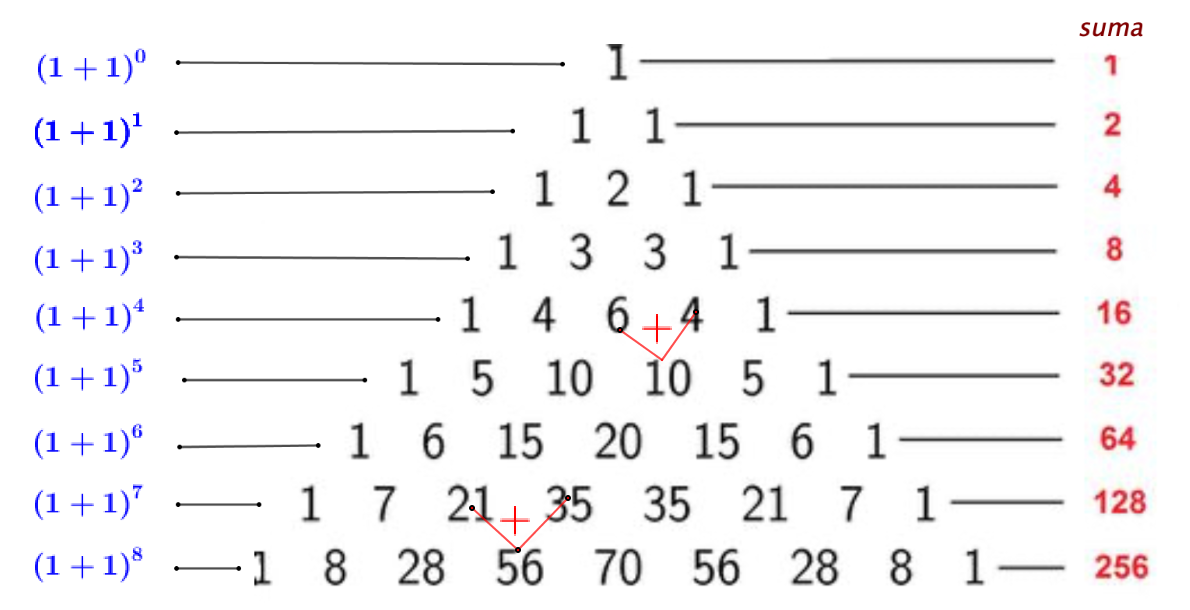
\includegraphics[width=0.75\textwidth]{img-reales/reales15.png}
	\end{figure}


\begin{theorem}[ Binomio de Newton]

$$(a+b)^n  = \mqty(n\\0)a^nb^0+\mqty(n\\1)a^{n-1}b^1+\mqty(n\\2)a^{n-2}b^2+ \cdots \mqty(n\\n-1)a^1b^{n-1}+\mqty(n\\n)a^0b^n $$

\vspace{2mm} Los coeficientes del desarrollo son los números de la fila $n$-ésima de Tartaglia.
	 
\end{theorem}




\begin{figure}[H]
	\centering
	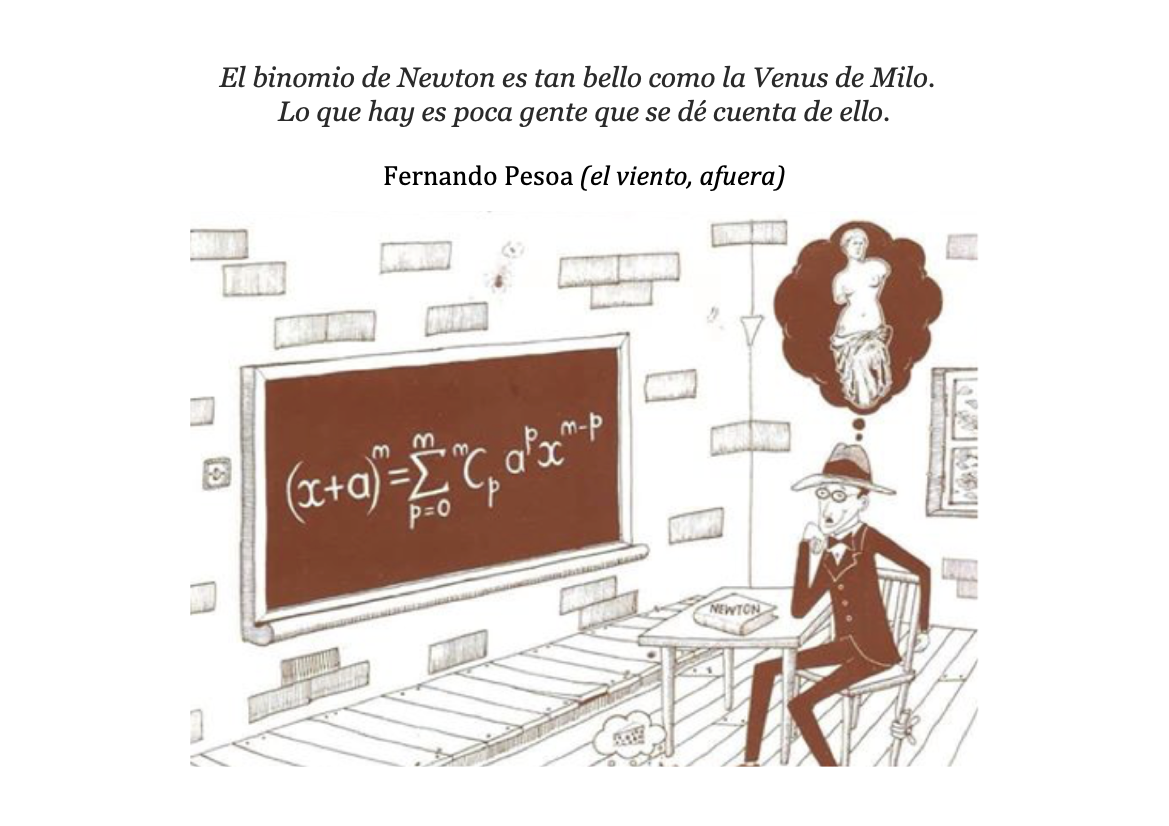
\includegraphics[width=0.85\textwidth]{img-reales/reales16.png}
	\end{figure}

\vspace{-10mm} %%%%%%%%%%%%%%%%%%%%%%
\begin{theorem}[ Propiedades del binomio de Newton]

\begin{enumerate}[1. ]
\item El término general del desarrollo es: $\ \ \mqty(n\\k)\, a^{n-k}\, b^k$

\textcolor{gris}{Si intercambianos $n-k$ por $k$, tenemos $\mqty(n\\n-k)\, a^k\, b^{n-k}\, . \ $ Los términos equidistantes del desarrollo tienen los mismos coeficientes.} 	

\item  Los coeficientes de $\, (a+b)^n \, $ son $\ \mqty(n\\0),\mqty(n\\1), \mqty(n\\2), \cdots , \mqty(n\\n)\, , \ $ coinciden con la fila $n$-sima del triangulo de tartaglia.

\item  La suma de los coeficientes del desarrollo de la potencia $n$-sima de un binomio es $\ 2^n$.

\textcolor{gris}{En efecto, si desarrollamos $(1+1)^n=2^n=\mqty(n\\0)+\mqty(n\\1)+\mqty(n\\2)+ \cdots + \mqty(n\\n)$}.

\end{enumerate}

\end{theorem}

	

\begin{miejercicio}

Calcular $(a-b)^4$

\rule{300pt}{0.1pt}

$(a-b)^4=[a+(-b)^4]$; los coeficientes serán los de la fila $4^a$ de Tartaglia, $\ 1,2,6,4,1$, así,

\vspace{2mm}$(a-b)^4=1a^4+4a^3(-b)+6a^2(-b)^2+4a(-b)^3+1(-b)^4=a^4-4a^3b+6a^2b^2-4ab^3+b^4$
	
\end{miejercicio}



\begin{miejercicio}

Calcula el término en $x^{12}$ del desarrollo de $(2x^2-1)^9$	

\rule{300pt}{0.1pt}

El término $k$-ésimo del desarrollo de $(a+b)^n$ es de la forma: $\  \mqty(n\\k) a^{n-k}b^k$

$(2x^2)^{9-k}2^{9-k}\, x^{2(9-k)} \ \to x^{18-2k}=x^{12} \ \to  18-2k=12 \ \to \ 6=2k \ \to \boldsymbol{k=3}$

Luego, el término buscado será:

$\mqty(9\\3)(2x^2)^{9-3}(-1)^3=\dfrac{9!}{3!\cdot 6!}(2x^2)^6(-1)=-\dfrac{9\cdot 8\cdot 7}{3\cdot 2} 2^6 x^{12} =-84\cdot 64x^{12}=\boldsymbol{ -5376x^{12} }$
\end{miejercicio}






\vspace{1cm}
\section{Ejercicios}

\begin{tikzpicture}
	\fill [left color=red!50, right color=teal!50] (0,0) rectangle (3.5,.1);
	\fill [left color=teal!50, right color=blue!50] (3.5,0) rectangle (7.5,.1);
	\end{tikzpicture}
\vspace{0.5cm}


\begin{mipropuesto}

Explica si estas frases son verdaderas o falsas:

\begin{enumerate}[a) ]
\item Hay números irracionales que son enteros.

\item Todo número irracional es real.

\item Todos los números decimales son racionales.

\item Entre dos números racionales hay infinitos números irracionales.

\item Todos los números decimales son racionales.

\item Entre dos enteros siempre hay un entero más.	
\end{enumerate}
\end{mipropuesto}

\vspace{-8mm}
\begin{flushright}
\begin{footnotesize} \textcolor{gris}{\rotatebox{180}{V: b, d}}	\end{footnotesize}
\end{flushright}


\begin{mipropuesto}

Escribe como intervalos:	 

\hspace{2cm} $a)\  \{x\in \mathbb R\, / \, -2\leq x \leq 3\}\,; \qquad b)\  \{x\in \mathbb R\, / \, -2< x \leq 3\}$

\hspace{2cm} $c)\  \{x\in \mathbb R\, / \, -2\leq x < 3\}\,; \qquad  d)\ \{x\in \mathbb R\, / \, -2< x < 3\}$

\hspace{2cm} $e)\  \{x\in \mathbb R\, / \,  x \leq 3\}\,; \quad \qquad \qquad  f)\ \{x\in \mathbb R\, / \,  x > -2 \}$
\end{mipropuesto}

\vspace{-8mm}
\begin{flushright}
\begin{footnotesize} \textcolor{gris}{\rotatebox{180}{ $\quad a)\ [-2,3]; \ \ b)\ ]-2,3]; \ \ c)\ [-2,3[; \ \ d)\ ]-2,3[; \ \ e)\ ]-\infty,3]; \ \ f)\ ]-2,+\infty[$ }}	\end{footnotesize}
\end{flushright}



\begin{mipropuesto}

Determina cuales son los números reales cuya distancia a $-1$ es menor que $2$.	
\end{mipropuesto}

\vspace{-8mm}
\begin{flushright}
\begin{footnotesize} \textcolor{gris}{\rotatebox{180}{$\{x\in \mathbb R \, / \, d(x,-1)<2\}\ = \ E_2(-1) \ \equiv \ ]-3,1[$}}	\end{footnotesize}
\end{flushright}

\begin{mipropuesto}

Introduce y extrae factores del radical.	

$\sqrt[3]{81\cdot 10^4\, x^6};\qquad \sqrt{\dfrac{16a^4}{27}} ;\qquad (x+1)\sqrt{\dfrac{x-1}{x+1}};\qquad \dfrac 2{x} \sqrt[3]{x^2} $
\end{mipropuesto}

\vspace{-8mm}
\begin{flushright}
\begin{footnotesize} \textcolor{gris}{\rotatebox{180}{$30x^2\sqrt{30};\qquad \dfrac{4a^2}{3\sqrt{3}};\qquad \sqrt{x^2-1};\qquad \sqrt[3]{\dfrac 8 x}$}}	\end{footnotesize}
\end{flushright}


\begin{mipropuesto}
	
	Calcula: $\quad \dfrac{8\sqrt{72}-3\sqrt{288}-2\sqrt{338}}{7\sqrt{2}} \qquad \qquad  -2\sqrt{\dfrac{20}{27}} +\sqrt{\dfrac{125}{3}}-\dfrac 6 5 \sqrt{\dfrac{45}{12}}-3 \sqrt{\dfrac 5 3}$
\end{mipropuesto}

\vspace{-8mm}
\begin{flushright}
\begin{footnotesize} \textcolor{gris}{\rotatebox{180}{$-2\, ; \qquad \qquad -\dfrac{17}{15}\sqrt{\dfrac{5}{3}}$}}	\end{footnotesize}
\end{flushright}


\begin{mipropuesto}
	
	Efectua las siguientes operaciones:
\begin{multicols}{2}	
	\begin{enumerate}[a) ]
	\item 	$\sqrt{\sqrt{a^2\cdot \sqrt[3]{a^2}}}$
	\item $\dfrac{\sqrt[3]{x^2y^2}\cdot \sqrt{xy}}{\sqrt[6]{x^11y^8}}$
	\item   $\sqrt[3]{(-1)^3\, \sqrt[5]{\sqrt[3]{-1}}}+1$
	\item $(1-2\sqrt{2})^2-(1+2\sqrt{2})^2$
	\item $(\sqrt{5}-2)\cdot (\sqrt{5}+2)+(2\sqrt{2})^2$
	\item $\sqrt{4+2\sqrt{3}}-\sqrt{4+2\sqrt{3}}\qquad (*)$
	\end{enumerate}
\end{multicols}
$f)\quad \sqrt{a^3-a^2b}+\sqrt{(a-b)(a^2-2ab+b^2)}+\sqrt{ab^2-b^3}$
\vspace{1mm}
\end{mipropuesto}



\vspace{-8mm}
\begin{flushright}
\begin{footnotesize} \textcolor{gris}{\rotatebox{180}{$a)\ \sqrt[3]{a};\quad b) \ \sqrt[6]{\dfrac{y^9}{x^4}};\quad c) \ 2;\quad d)\  -8\sqrt{2};\quad e)\  9;\quad f) \ 2a\sqrt{a-b}$}}	\end{footnotesize}
\end{flushright}

\vspace{-8mm}
\begin{flushright}
\begin{footnotesize} \textcolor{gris}{\rotatebox{180}{$e)\ (*)\ $ eleva, previamente, al cuadrado.}}	\end{footnotesize}
\end{flushright}

\begin{mipropuesto}
	
	Calcula: $\quad a)\ \ \dfrac{3}{\sqrt{3}-\sqrt{2}} - \dfrac{2}{\sqrt{3}+\sqrt{2}}\, ; \qquad\qquad b) \ \ \dfrac{\sqrt{7}-\sqrt{5}}{\sqrt{7}+\sqrt{5}}-\dfrac{\sqrt{7}+\sqrt{5}}{\sqrt{7}-\sqrt{5}}$

\end{mipropuesto}

\vspace{-8mm}
\begin{flushright}
\begin{footnotesize} \textcolor{gris}{\rotatebox{180}{$a)\ 3+5\sqrt{2}; \qquad b)\ -2\sqrt{35} $}}	\end{footnotesize}
\end{flushright}


\begin{mipropuesto}
	
	Racionaliza:
	
	\begin{multicols}{2}
	\begin{enumerate}[a) ]
	\item 	$\dfrac{1-\sqrt{3}}{2\sqrt{3}}$
	\item $\left( \dfrac{x^2}{\sqrt{x^3}} \right)^2$
	\item $\dfrac{\sqrt{x}+\sqrt{y}}{\sqrt{x}-\sqrt{y}}$
	\item $\dfrac{3+2\sqrt{5}}{2\sqrt{3}-\sqrt{6}}$
	\end{enumerate}
	\end{multicols}
	\vspace{1mm}
\end{mipropuesto}

\vspace{-8mm}
\begin{flushright}
\begin{footnotesize} \textcolor{gris}{\rotatebox{180}{$a)\ \dfrac{\sqrt{3}-6}{6};\qquad b)\ x;\qquad c)\ \dfrac{x+y+2\sqrt{xy}}{x-y};\qquad d)\ 2+\sqrt{2}+\sqrt{3}+ \dfrac {\sqrt{6}}{2} $}}	\end{footnotesize}
\end{flushright}

\begin{mipropuesto}
	
	Calcula:	
$\quad a)\ \dfrac{\sqrt
24-\sqrt{150}+4\sqrt{54}}{\sqrt{6}};\qquad \qquad \qquad b)\ \dfrac{\sqrt{3}}{2\sqrt{3}-2}-\dfrac{5}{\sqrt{3}+3}+\dfrac{2}{\sqrt
{3}}$
\end{mipropuesto}

\vspace{-8mm}
\begin{flushright}
\begin{footnotesize} \textcolor{gris}{\rotatebox{180}{$a)\ 9;\quad b) \dfrac{21}{12}(\sqrt{3}-1)$}}	\end{footnotesize}
\end{flushright}


\begin{mipropuesto}
	
	Calcula:
\begin{multicols}{2}	
\begin{enumerate}[a) ]
	\item $\log_2 0.25$
	\item $\mathrm{Log}\, 0.001$
	\item $\log_4 2$
	\item $\log_9 27$
	\item $\log_3 0.333\cdots$
	\item $\log_3 \dfrac{2}{54}$
	\item $\log_{0.01}100$
	\item $\log_{1/8} \dfrac 1 4$
\end{enumerate}
\end{multicols}	
\vspace{1mm}
\end{mipropuesto}

\vspace{-8mm}
\begin{flushright}
\begin{footnotesize} \textcolor{gris}{\rotatebox{180}{$a)\ -2;\quad b)\  -3;\quad c) 1/2;\quad d) \ 3/2;\quad e)\ -1;\quad f) -3;\quad g) -1;\quad h) \ -2/3$}}	\end{footnotesize}
\end{flushright}

\begin{mipropuesto}

Calcula: $\quad \log_6 x=2.5$	
\end{mipropuesto}

\vspace{-8mm}
\begin{flushright}
\begin{footnotesize} \textcolor{gris}{\rotatebox{180}{$36\sqrt{6}$}}	\end{footnotesize}
\end{flushright}

\begin{mipropuesto}
	
	Calcula:

\begin{multicols}{2}	
\begin{enumerate}[a) ]
	\item $\log_3 7\cdot \log_7 3$
	\item $-\log_3 5 \cdot \log_5 9$
	\item $\log_7(\log_3(\log_2 8)))$
	\item $\log_4(\log_2(\log_3(10-\mathrm{Log}\, 10)))$
\end{enumerate}
\end{multicols}
\vspace{1mm}	

\end{mipropuesto}

\vspace{-8mm}
\begin{flushright}
\begin{footnotesize} \textcolor{gris}{\rotatebox{180}{$a)\ 1;\qquad b)\ -2;\qquad c)\ 0;\qquad d)\ 0$}}	\end{footnotesize}
\end{flushright}

\vspace{-8mm}
\begin{flushright}
\begin{footnotesize} \textcolor{gris}{\rotatebox{180}{El cambio de base de los logaritmos puede serte útil.}}	\end{footnotesize}
\end{flushright}


\begin{mipropuesto}

Demuestra que: 
$\qquad a)\ \ \log_ba\, \log_db\, \log_ed=\log_ea\, ; \qquad b)\ \ \log_ba=\dfrac{1}{\log_ab}$ 	
\end{mipropuesto}

\vspace{-8mm}
\begin{flushright}
\begin{footnotesize} \textcolor{gris}{\rotatebox{180}{a) escribe toco con $\log_e$; $\qquad$  b) déjalo todo con $\log_a$.}}	\end{footnotesize}
\end{flushright}


\begin{mipropuesto}

$(x+1)^{\log(x+1)}=100(x+1)$	
\end{mipropuesto}

\vspace{-8mm}
\begin{flushright}
\begin{footnotesize} \textcolor{gris}{\rotatebox{180}{ Tomando logaritmos decimales se llega a una ecuación de segundo grado en $\log(x+1)$}}	\end{footnotesize}
\end{flushright}



\begin{mipropuesto}

?`Es cierta la siguiente igualdad? $\qquad \log(a^2-b^2)=\log(a\cdot b)+\log \left( \dfrac a b - \dfrac b a \right)$ 	
\end{mipropuesto}

\vspace{-8mm}
\begin{flushright}
\begin{footnotesize} \textcolor{gris}{\rotatebox{180}{ Basta con operar y aplicar propiedades de los logaritmos. }}	\end{footnotesize}
\end{flushright}

\begin{mipropuesto}
	
Calcula:

\vspace{2mm} $a) \ \dfrac{12(k-2)!}{k!}; \qquad b)\ \mqty(k\\k-2)=10;\qquad c)\ 3\mqty(k\\4)=5\mqty(k\\2);\qquad d) \ \dfrac{(k+6)!}{(k+4)!}=72$

\end{mipropuesto}


\vspace{-8mm}
\begin{flushright}
\begin{footnotesize} \textcolor{gris}{\rotatebox{180}{$a)\ 4;\qquad b)\ 5;\qquad c)\ 7;\qquad d)\ 3$}}	\end{footnotesize}
\end{flushright}


\begin{mipropuesto}
	
	Calcula el octavo término del desarrollo $\ (x^2-3y^3)^{10}$	

\end{mipropuesto}

\vspace{-8mm}
\begin{flushright}
\begin{footnotesize} \textcolor{gris}{\rotatebox{180}{El octavo término se alcanza con $k=7;\qquad -262440x^6y^{21}$}}	\end{footnotesize}
\end{flushright}



\begin{mipropuesto}
	
	Calcula el término independiente de $\ \left( a^3-\dfrac{2}{a} \right)^{20} $	

\end{mipropuesto}

\vspace{-8mm}
\begin{flushright}
\begin{footnotesize} \textcolor{gris}{\rotatebox{180}{El término independiente es $\ x^0;\qquad -208\, 035\, 0721$}}	\end{footnotesize}
\end{flushright}

\begin{mipropuesto}

Desarrolla: $\quad \left( \sqrt{\dfrac 2 x }+\sqrt{2x} \right)^2$	
\end{mipropuesto}

\vspace{-8mm}
\begin{flushright}
\begin{footnotesize} \textcolor{gris}{\rotatebox{180}{$16 \; x^{4} + 128 \; x^{3} + 448 \; x^{2} + 896 \; x^{1} + 1120 \; + 896 \; x^{-1} + 448 \; x^{-2} + 128 \; x^{-3} + 16 \; x^{-4}$}}	\end{footnotesize}
\end{flushright}









\newpage

\begin{adjustwidth}{50pt}{250pt}
\begin{cuadro-naranja}
\textbf{\huge{Problemas $\boldsymbol{+}$}}\normalsize{$\, $}
\end{cuadro-naranja}	
\end{adjustwidth}

\vspace{2mm}
\begin{enumerate}[\textbf{P$\boldsymbol +$} 1. ]
\item	?`Qué falla en la siguiente demostración?

\begin{multicols}{2}
\begin{enumerate}
\item $4=4$
\item $4\cdot(-5)=4\cdot(-5)$
\item $-20=-20$
\item $16-36=25-45$
\item $16-36+\dfrac {81} 4=25-45+\dfrac {81} 4$
\item $\left(4-\dfrac 9 2 \right)^2=\left(5-\dfrac 9 2 \right)^2$
\item $4-\dfrac 9 2 = 5-\dfrac 9 2$
\item $\boxed{ \ \boldsymbol{4\ = \ 5} \ } $ 

\QED
\end{enumerate}
\end{multicols}
\vspace{-6mm}
\begin{flushright}
\begin{footnotesize} \textcolor{gris}{\rotatebox{180}{En el paso f) a g) no se han tomado valores absolutos.}}	\end{footnotesize}
\end{flushright}

\item Calcula: $\quad a)\ 27^{\widehat{0.3}};\qquad b)\ \sqrt[3]{8^{27x^3}}$
\vspace{-6mm}
\begin{flushright}
\begin{footnotesize} \textcolor{gris}{\rotatebox{180}{Escribe como potencias de exponente racional. $\qquad a) \ 3;\quad b) \ 8^{9x^3} $ }}	\end{footnotesize}
\end{flushright}

\item Calcula: $\quad  a) \ \dfrac{\sqrt{2}+\sqrt{6}}{\sqrt{2+\sqrt{3}}} ;\qquad b)\  \sqrt{4+\sqrt{7}}-\sqrt{4-\sqrt{7}} ;\qquad c)\ \sqrt{4+\dfrac{\sqrt{63}}{2}}+\sqrt{4-\dfrac{\sqrt{63}}{2}}$ 

\vspace{-6mm}
\begin{flushright}
\begin{footnotesize} \textcolor{gris}{\rotatebox{180}{Eleva al cuadrado previamente. $\qquad a) \ 2;\quad b) \ 	\sqrt{2};\quad c)\ 3 $ }}	\end{footnotesize}
\end{flushright}

\item Sean $\ x=\dfrac{\sqrt{3}-\sqrt{2}}{\sqrt{3}+\sqrt{2}}  \ \ \text{ e } \ \ y=\dfrac{\sqrt{3}+\sqrt{2}}{\sqrt{3}-\sqrt{2}}\, , \  $  calcula $\ \ x^2+xy+y^2$

\vspace{-6mm}
\begin{flushright}
\begin{footnotesize} \textcolor{gris}{\rotatebox{180}{$99$ }}	\end{footnotesize}
\end{flushright}

\item Calcula $\ (log_2 3)\,(log_3 4)\,(log_3 5)\,(log_6 6)\, \cdot (log_{511} 512)$

\vspace{-6mm}
\begin{flushright}
\begin{footnotesize} \textcolor{gris}{\rotatebox{180}{Escríbelo todo como $\log_2\qquad $ sol.: 9 }}	\end{footnotesize}
\end{flushright}

\item Calcula $\ a)\ \text{ si } \ \log_2x=3 \ \to \ \text{ calcula }\ \log_x 64;\qquad \qquad b)\ 3\log_8 x=\log_4(x+6)$

\vspace{-6mm}
\begin{flushright}
\begin{footnotesize} \textcolor{gris}{\rotatebox{180}{Escríbelo todo como $\log_2\ \  $ sol.: $\ a)\ 2;\qquad  b)\ 3$ }}	\end{footnotesize}
\end{flushright}

\item Resuelve: $\quad a)\ 4^{\log_{16}{25}}=x;\qquad b)\ \log_{\log_3 9}8_x ;\qquad c)\ \ln{e^{\ln{(e^e)}}}=x$

\vspace{-6mm}
\begin{flushright}
\begin{footnotesize} \textcolor{gris}{\rotatebox{180}{Recuerda que $\ \log_a a^x=x=a^{\log_a x}\ \qquad \text{ sol.: }\  a)\ 25;\qquad b)\ 3;\qquad c)\ e$ }}	\end{footnotesize}
\end{flushright}

\item Calcula $\quad \log_2 x+\log_2 \sqrt{x} + \log_2 \sqrt{\sqrt{x}}+\log_2  \sqrt{\sqrt{\sqrt{x}}} +\, \cdots \, = \, 4 $

\vspace{-6mm}
\begin{flushright}
\begin{footnotesize} \textcolor{gris}{\rotatebox{180}{Recuerda la suma de infinitos términos de una progresión geométrica $\ \ [\, S_\infty=a_1/(1-r)\, ]\qquad $ sol.: $4$ }}	\end{footnotesize}
\end{flushright}

\item Prueba que $\ \dfrac{1}{\log_aabc}+\dfrac{1}{\log_babc}+\dfrac{1}{\log_cabc}=1$

\vspace{-6mm}
\begin{flushright}
\begin{footnotesize} \textcolor{gris}{\rotatebox{180}{ Escribe todos los logaritmos en la misma base. }}	\end{footnotesize}
\end{flushright}

\item Prueba que $\ \dfrac{1}{\log_\pi e}+\dfrac{1}{\log_e \pi}>2$

\vspace{-6mm}
\begin{flushright}
\begin{footnotesize} \textcolor{gris}{\rotatebox{180}{ solo tienes que escribir como cuadrado perfecto. }}	\end{footnotesize}
\end{flushright}

\vspace{-8mm}
\begin{flushright}
\begin{footnotesize} \textcolor{gris}{\rotatebox{180}{ Has de demostrar que $x+\dfrac 1 x >2$, con $x>0$, }}	\end{footnotesize}
\end{flushright}

\vspace{-8mm}
\begin{flushright}
\begin{footnotesize} \textcolor{gris}{\rotatebox{180}{ Escribe todos los logaritmos en la misma base. }}	\end{footnotesize}
\end{flushright}

\item Si el radio de una circunferencia de longitud  $\ \log b 4\ $ es $\ \log a^4\, , \ $ ?`Cuál es el valor de $\ \log_a b\, $?

\vspace{-6mm}
\begin{flushright}
\begin{footnotesize} \textcolor{gris}{\rotatebox{180}{ Longitud circunferencia = 2$\pi$ radio. \qquad sol: $\pi$}}	\end{footnotesize}
\end{flushright}

\item $\dfrac{1}{\log_2 a}+\dfrac{1}{\log_3 a}+\dfrac{1}{\log_4 a}=1\ $ ?`Cuál es el valor de $\ a\, $?

\vspace{-6mm}
\begin{flushright}
\begin{footnotesize} \textcolor{gris}{\rotatebox{180}{ Escribe todo en la misma base. $\qquad$ sol: $\ a=24$ }}	\end{footnotesize}
\end{flushright}

\item Calcula $\quad \dfrac{1}{\log_2(100!)}+\dfrac{1}{\log_3(100!)}+\dfrac{1}{\log_4(100!)}+\cdots +\dfrac{1}{\log_100(100!)}$

\vspace{-4mm}
\begin{flushright}
\begin{footnotesize} \textcolor{gris}{\rotatebox{180}{ Escribe todo en la misma base. $\qquad$ sol: $\ 1$ }}	\end{footnotesize}
\end{flushright}

\end{enumerate}

\newpage

\section{Resumen del tema}

\begin{tikzpicture}
	\fill [left color=red!50, right color=teal!50] (0,0) rectangle (3.5,.1);
	\fill [left color=teal!50, right color=blue!50] (3.5,0) rectangle (7.5,.1);
	\end{tikzpicture}
\vspace{0.5cm}

\begin{myblock}{ Resumen \emph{`Números reales'}}

\begin{figure}[H]
	\centering
	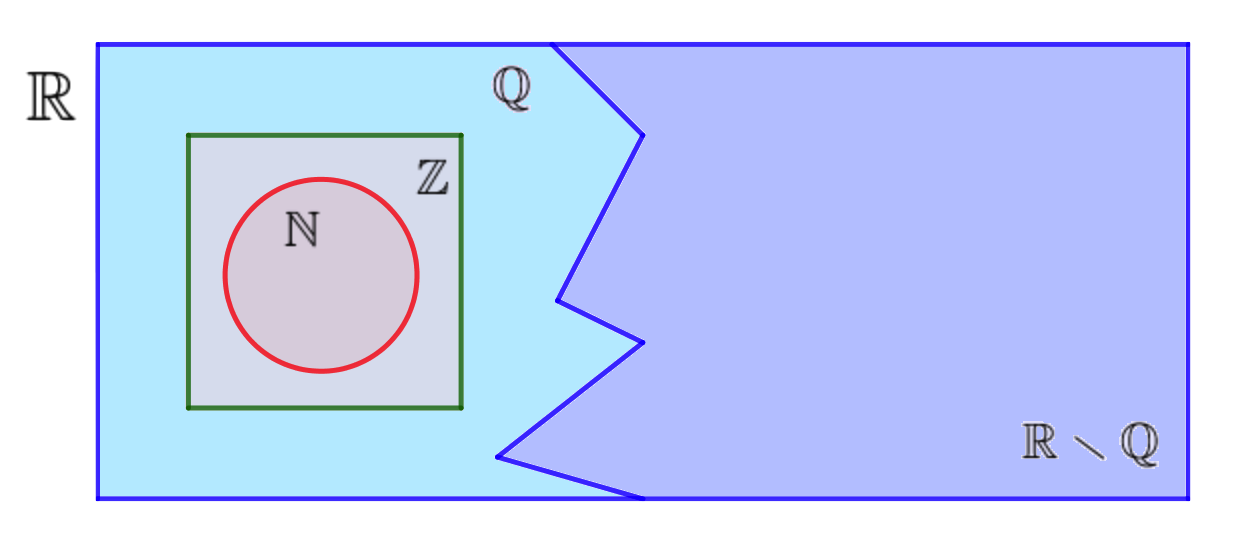
\includegraphics[width=0.75\textwidth]{img-reales/reales18.png}
	\end{figure}
	
\begin{table}[H]
\centering
\small
\begin{tabular}{|c|c|c|c|}
\hline
$|x|=\begin{cases} \  x & \text{ si } x\geq 0 \\  -x & \text{ si } x<0 \end{cases}$  & $[a,b[ \equiv \{\forall x \in \mathbb R \, / \, a\leq x < b \}$ & $d(x,y)=|x-y|$ & $E_r(a)=]a-r,a+r[$ \\ \hline
\end{tabular}
\end{table}

\vspace{5mm}
\begin{table}[H]
\centering
\begin{tabular}{|c|}
\hline
$\boldsymbol{ \sqrt[n]a \ = \ b \ \ \leftrightarrow \ \ b\ = \ a^n } \, ; \qquad a,b \in \mathbb R; \quad n\in \mathbb N\, , \ n>1$
 \\ \hline
\end{tabular}
\end{table}

\begin{table}[H]
\centering
\begin{tabular}{|c|c|c|}
\hline
$\sqrt[n]a^m=a^{m/n}$ & $\sqrt[n]{a} \, \cdot \, : \, \sqrt[n]{b} = \sqrt[n]{a\,  \cdot \, : \,  b}$ & $(\sqrt[n]{a})^m=\sqrt[n]{a^m}$ \\  \hline
$\sqrt[n]{\sqrt[m]{a}}=\sqrt[n\cdot m]{a}$ & $\sqrt[n]{a^m}=\sqrt[n\cdot k]{a^{m\cdot k}}$ & $b\sqrt[n]{a}=\sqrt[n]{b^n\, a}$ \\ \hline
\end{tabular}
\end{table}

\begin{table}[H]
\centering
\begin{tabular}{|c|c|c|}
\hline
Denominador & Factor racionalizante & Denominador racionalizado \\ \hline
$\sqrt[n]a^m$ & $\sqrt[n]a^{n-m}$ & $a$ \\ \hline
$\sqrt{a} \pm \sqrt{b}$ & $\sqrt{a} \mp \sqrt{b}$ & $a-b$ \\ \hline
\end{tabular}
\end{table}	

\vspace{5mm}

\begin{table}[H]
\centering
\begin{tabular}{|c|}
\hline
$\boldsymbol{ \log_aP\ = \ b \ \ \leftrightarrow \ \ a^P\ = \ b } \, ; \qquad a>0 \, \wedge \, a\neq 1 ;\quad P>0$
 \\ \hline
\end{tabular}
\end{table}

\begin{table}[H]
\centering
\begin{tabular}{|c|c|c|}
\hline
$\log_aa=1$ & $\log_a1=0$ & $\log_a(A\cdot B)=\log_aA+\log_aB$ \\ \hline
$\log_a(A / B)=\log_aA-\log_aB$ & $\log_aA^n=n\, \log_aA$ & $\log_bP=\dfrac{\log_aP}{\log_ab}$ \\ \hline
\end{tabular}
\end{table}	
\vspace{5mm}

\begin{table}[H]
\centering
\begin{tabular}{|c|}
\hline
  $(a+b)^n  = \mqty(n\\0)a^nb^0+\mqty(n\\1)a^{n-1}b^1+\mqty(n\\2)a^{n-2}b^2+ \cdots \mqty(n\\n-1)a^1b^{n-1}+\mqty(n\\n)a^0b^n $ \\ \hline
\end{tabular}
\end{table}
\end{myblock}












\begin{comment}	



%%%%%%%%%%%%%%%%%%%%%%%%%%%%%%%%%%%. SECCIONES
\chapter{texto}

\begin{tikzpicture}
	\fill [left color=red!50, right color=teal!50] (0,0) rectangle (6.5,.2);
	\fill [left color=teal!50, right color=blue!50] (6.5,0) rectangle (11.5,.2);
	\end{tikzpicture}

\vspace{1cm}
\section{texto}

\begin{tikzpicture}
	\fill [left color=red!50, right color=teal!50] (0,0) rectangle (3.5,.1);
	\fill [left color=teal!50, right color=blue!50] (3.5,0) rectangle (7.5,.1);
	\end{tikzpicture}
\vspace{0.5cm}

\subsection{texto}

\begin{tikzpicture}
	\fill [left color=red!50, right color=teal!50] (0,0) rectangle (3.5,.01);
	\fill [left color=teal!50, right color=blue!50] (3.5,0) rectangle (7.5,.01);
	\end{tikzpicture}
\vspace{0.5cm}


%$$$$$$$$$$$$$$$$$$$$$$$$$$$$$$$$$$$$$$$$$$$$$$$$$$$$$$$$$
\begin{mipropuesto}
	
	Calcula	

\end{mipropuesto}

\vspace{-8mm}
\begin{flushright}
\begin{footnotesize} \textcolor{gris}{\rotatebox{180}{E}}	\end{footnotesize}
\end{flushright}
%$$$$$$$$$$$$$$$$$$$$$$$$$$$$$$$$$$$$$$$$$$$$$$$$$$$$$$$$$

%%%%%%%%%%%%%%%%%%%%%%%%%%%%%%%%%%%. \begin{ ------>. 
detsacado;  cuadro-naranja;  cuadro-gris;  miejercicio (solución extensa);  mipropuesto (solución corta y fuera del cuadro)

%%%%%%%%%%%%%%%%%%%%%%%%%%%%%%%%%%%. CURIOSIDAD
\vspace{1cm}
\color{ForestGreen!80}
\rule{250pt}{0.2pt}
Texto
\vspace{-8mm}
\begin{flushright}
\rule{250pt}{0.2pt}		
\end{flushright}	
\color{black}
\end{comment}